\documentclass[preprint,12pt]{elsarticle}

% ---------------- Packages ----------------
\usepackage{amsmath,amssymb,amsfonts}
\usepackage{graphicx}
\usepackage{textcomp}
\usepackage{xcolor}
\usepackage{multirow}
\usepackage{booktabs}
\usepackage{array}
\usepackage{ragged2e}
\usepackage{siunitx}
\usepackage{url}
\usepackage{bm}
\usepackage{lineno}
\usepackage{hyperref}

\journal{Journal Name}

\begin{document}

\begin{frontmatter}

% ---------------- Title ----------------
\title{DLC-Enhanced TiO$_2$-Au-Coated Slotted PCF-SPR Sensor for Wide-Range Refractive Index Detection}

% ---------------- Authors ----------------
\author[inst1]{Md. Tajmimul Islam Soumik}
\ead{tajmimulsoumik008@gmail.com}

\affiliation[inst1]{organization={Department of Electronics and Telecommunication Engineering, Rajshahi University of Engineering \& Technology (RUET)},
            city={Rajshahi},
            country={Bangladesh}}

% ---------------- Abstract ----------------
\begin{abstract}
A diamond-like carbon (DLC)-enhanced TiO$_2$-Au-coated slotted photonic crystal fiber surface plasmon resonance (PCF-SPR) sensor is proposed for wide-range refractive index (RI) detection. The sensing performance of the proposed structure is numerically investigated over the analyte RI range of 1.33-1.41 using the finite element method. To evaluate the influence of DLC coating, the sensor response is compared with and without the DLC layer. The results show that the DLC-coated structure provides improved overall sensing performance over most of the investigated RI range, particularly from 1.33 to 1.39, compared with the uncoated structure. By incorporating the DLC layer, the proposed sensor achieves a maximum wavelength sensitivity of 13000 nm/RIU, a maximum amplitude sensitivity of -1768.4 RIU$^{-1}$, and a minimum detection resolution in the order of 10$^{-6}$ RIU. The performance enhancement is mainly attributed to stronger plasmonic coupling between the core-guided mode and the surface plasmon polariton mode induced by the TiO$_2$-Au-DLC coating. Therefore, the proposed DLC-assisted PCF-SPR sensor can be considered a promising candidate for wide-range RI sensing applications.
\end{abstract}

% ---------------- Keywords ----------------
\begin{keyword}
Photonic crystal fiber \sep surface plasmon resonance \sep refractive index sensor \sep diamond-like carbon \sep TiO$_2$ \sep gold \sep finite element method
\end{keyword}

\end{frontmatter}

% ---------------- Introduction ----------------
\section{\textbf{{Introduction}}}

Accurate refractive-index (RI) sensing is very important in biomedical analysis, chemical detection, environmental monitoring, and food-safety inspection. Many biological and chemical samples produce only small changes in RI, so a sensor must detect these changes clearly and reliably. This is especially important for disease diagnosis, because cancer cells, infected red blood cells, exosomes, blood components, bacteria, and other biomolecules often have very close RI values. Surface plasmon resonance (SPR) is widely used for label-free RI sensing because it gives a strong optical response at the metal--analyte interface. Photonic crystal fiber (PCF) is also a useful platform because its air-hole arrangement, core position, sensing channel, and coating layers can be designed to improve the interaction between light and the analyte \cite{chaity2024highly,ashrafian2025highly,guo2025dual,khatun2025design}.

In recent years, many PCF-SPR sensors have been proposed for cancer-cell detection. Chaity proposed a single-core circular PCF-SPR biosensor for six different cancer cells and reported a maximum wavelength sensitivity of 8571.42 nm/RIU, amplitude sensitivity of -2589.15 RIU$^{-1}$, and FOM of 263.73 RIU$^{-1}$ \cite{chaity2024highly}. Ashrafian \emph{et al.} designed an open D-channel PCF-SPR biosensor using Au and TiO$_2$ layers for cancer-cell detection. In their cancer-cell analysis, the highest wavelength sensitivity was 5214.285 nm/RIU, with amplitude sensitivity of -1481.1 RIU$^{-1}$, resolution of $1.19 \times 10^{-5}$ RIU, and FOM of 350 RIU$^{-1}$ \cite{ashrafian2025highly}. Akter and Abdullah developed a gold-coated circular PCF-SPR biosensor for different cancer cells, while Jamil \emph{et al.} used Au and TiO$_2$ layers for early breast-cancer detection in the near-infrared region \cite{akter2025design,jamil2025gold}. These studies show that PCF-SPR sensors are very promising for identifying different cancer cells through their RI variation.

Several works have also focused on improving the structure and material layers of PCF-SPR sensors. Guo \emph{et al.} proposed a U-shaped Au-TiO$_2$ coated PCF-SPR sensor for dual-polarization RI detection and reported maximum wavelength sensitivities of 10,200 nm/RIU and 5900 nm/RIU for two polarization ranges \cite{guo2025dual}. Debbarma \emph{et al.} introduced a tetrad-channel PCF-SPR biosensor for the simultaneous detection of blood, breast, cervical, and adrenal gland cancers. Their design shows how multi-channel structures can be used for parallel cancer detection in a single sensing platform \cite{debbarma2026tetrad}. Cui \emph{et al.} also developed a dual-polarization four-channel PCF-SPR sensor with wide RI detection range and high linearity, showing the importance of polarization control and channel separation in advanced PCF-SPR designs \cite{cui2026high}. Paul \emph{et al.} used a DLC-TiO$_2$-Au multilayer D-shaped structure for cancer-cell detection and showed that DLC-based multilayer coating can strongly improve the sensing response and resolution \cite{paul2025dlc}.

PCF-SPR sensors have also been applied beyond cancer-cell detection. Azadi \emph{et al.} proposed a D-shaped TiO$_2$--Au hybrid PCF-SPR biosensor for blood-constituent detection, showing the ability of PCF-SPR sensors to distinguish samples with close RI values \cite{azadi2025ultrahigh}. Tayef \emph{et al.} designed a D-shaped Au/TiO$_2$ coated PCF-SPR biosensor for early malaria detection by analyzing different infected red-blood-cell phases \cite{tayef2025highly}. Ji \emph{et al.} reported a Ge-doped PCF-SPR biosensor for tumor-cell exosome detection over a wide RI range, which is important for early disease monitoring \cite{ji2026high}. Oyon \emph{et al.} studied balanced geometry selection in circular PCF-SPR biosensors for cancer and bacterial detection, where the design reached a highest wavelength sensitivity of 20,714 nm/RIU but mainly emphasized the role of balanced structural optimization \cite{oyon2026numerical}. These studies confirm that PCF-SPR sensors can be adapted for different biomedical targets by changing the geometry, coating layers, and sensing region.

The application range of PCF-SPR sensors has also expanded to environmental, chemical, and food-quality monitoring. Zheng \emph{et al.} proposed a dual-side polished PCF-SPR sensor for independent humidity and temperature monitoring, where separate sensitive materials were used to reduce cross-sensitivity \cite{zheng2026high}. Guo \emph{et al.} developed a coaxial dual-metal PCF-SPR sensor for simultaneous pathogen and body-temperature detection, showing the usefulness of combining different plasmonic regions in one fiber structure \cite{guo2026dual}. Sultana \emph{et al.} designed a PCF-SPR sensor for detecting fat and melamine in milk and reported a peak wavelength sensitivity of 7000 nm/RIU over the RI range of 1.22-1.38 \cite{sultana2026design}. Rabiei \emph{et al.} proposed a D-shaped hybrid grating SPR sensor using gold, TiO$_2$, and silver layers, and reported a sensitivity of 5100 nm/RIU, FWHM of about 14.5 nm, and FOM of 351.7 RIU$^{-1}$ \cite{rabiei2026high}. These works show that PCF-SPR sensors are not limited to medical diagnosis only; they can also be used in environmental and quality-control applications.

Material selection plays a major role in improving PCF-SPR sensor performance. Gold is widely used as the main plasmonic material because it gives a stable SPR response. TiO$_2$ is often used between gold and silica because it improves adhesion and helps tune the resonance condition \cite{ashrafian2025highly,guo2025dual,azadi2025ultrahigh,jamil2025gold}. Aravindhan \emph{et al.} reported a TiO$_2$-Au coated multihole PCF-SPR biosensor and achieved a peak wavelength sensitivity of 11,428.57 nm/RIU, amplitude sensitivity of 1917.6 RIU$^{-1}$, resolution of $1.2 \times 10^{-5}$ RIU, and FOM of 404.27 \cite{aravindhan2026design}. Nandhagopal \emph{et al.} used an Au--graphene hybrid interface in a dual-mode D-shaped PCF-SPR sensor and obtained a sensitivity of 1766 nm/RIU, FWHM of 10.4 nm, and FOM of 169.8 RIU$^{-1}$ \cite{nandhagopal2026highly}. Maurya \emph{et al.} also used a graphene-gold hybrid coating in a dual-core PCF-SPR biosensor, showing that hybrid material layers can improve light-matter interaction and sensing stability \cite{maurya2026ultra}. These studies indicate that proper coating selection is essential for improving resonance strength, linewidth, FOM, and overall sensing performance.

Although PCF-SPR sensors have shown strong sensing capability, limitations such as narrow RI coverage, complex structures, and reduced practical stability still exist. In this work, DLC is employed as an outer layer over the TiO$_2$-Au coating because of its chemical stability, biocompatibility, contamination resistance, and strong adhesion with TiO$_2$, which can improve the durability of the sensing interface \cite{paul2025dlc}. The DLC layer also strengthens the coupling between the core-guided mode and the surface plasmon mode, resulting in improved resonance shift and sensitivity. Hence, a DLC-assisted TiO$_2$-Au-coated PCF-SPR sensor is investigated for wide-range RI detection with clear resonance response and enhanced sensing performance.

Motivated by these aspects, a DLC-assisted TiO$_2$-Au-coated PCF-SPR sensor is proposed for broad-range refractive index sensing. In the multilayer structure, TiO$_2$ acts as the bottom adhesive and resonance-tuning layer, Au serves as the middle plasmonic layer, and DLC is used as the outer protective layer. The inclusion of DLC noticeably improves the sensing performance by enhancing the core-guided mode and surface plasmon mode interaction. As a result, the maximum wavelength sensitivity increases from 10,000 nm/RIU without DLC to 13,000 nm/RIU with DLC over the wide RI range of 1.33-1.41. Therefore, the proposed TiO$_2$-Au-DLC-based PCF-SPR sensor offers improved sensitivity, stable sensing behavior, and strong potential for practical RI detection applications.
% ---------------- Design and Method ----------------
\section{\textbf{{Sensor Design and Numerical Method}}}



\subsection{\textbf{{PCF Structure With Initial Design Parameters}}}

The schematic model and the sectional diagram of the proposed TiO$_2$-Au-DLC coated slotted PCF-SPR sensor are illustrated in Fig. 1. In the proposed structure, 17 circular air holes are arranged around the core region to support the fundamental core mode and to reduce unwanted light leakage. The circular air holes have a diameter of $d = 3~\mu$m and are separated by a pitch of $P = 2.5~\mu$m.

To guide the evanescent field toward the plasmonic sensing region, a rectangular-shaped coating region is introduced at the upper portion of the PCF structure. In this region, TiO$_2$, Au, and DLC layers are placed sequentially to facilitate the interaction between the surface plasmon polariton (SPP) mode and the fundamental core mode of the sensor. The rectangular TiO$_2$ layer is positioned at a distance of $D = 12~\mu$m from the center of the PCF.

The initial thicknesses of the three coating materials are selected as $t_{\mathrm{TiO_2}} = 10$ nm, $t_{\mathrm{Au}} = 45$ nm, and $t_{\mathrm{DLC}} = 9$ nm. The TiO$_2$ layer is used to improve the coupling condition between the guided core mode and the gold plasmonic layer, while the Au layer is employed to excite the SPR effect. In addition, the DLC layer is introduced over the plasmonic region to enhance the interaction between the evanescent field and the analyte medium.

The analyte is placed near the coated sensing region so that a change in the analyte refractive index can modify the phase-matching condition between the core-guided mode and the SPP mode. The proposed design is initially investigated over the analyte refractive index range of 1.33-1.41. These design parameters are further analyzed and adjusted in the optimization part to obtain improved sensing performance.

\begin{figure}[!t]
    \centering
    
    % ----------- 3D model -----------
    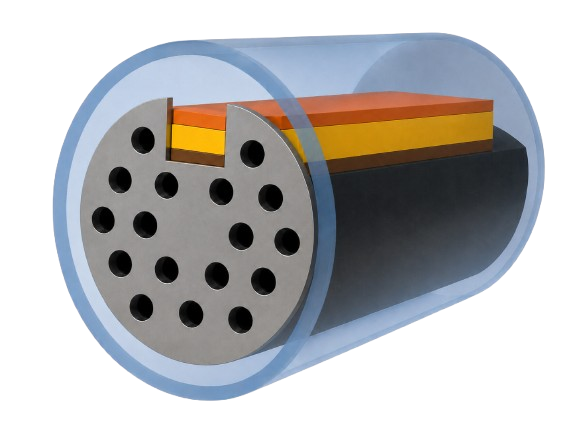
\includegraphics[width=0.5\textwidth]{main_3D_design-removebg-preview.png}
    
    \vspace{-1mm}
    {\small (a)}
    
    \vspace{2mm}
    
    % ----------- 2D cross-sectional diagram -----------
    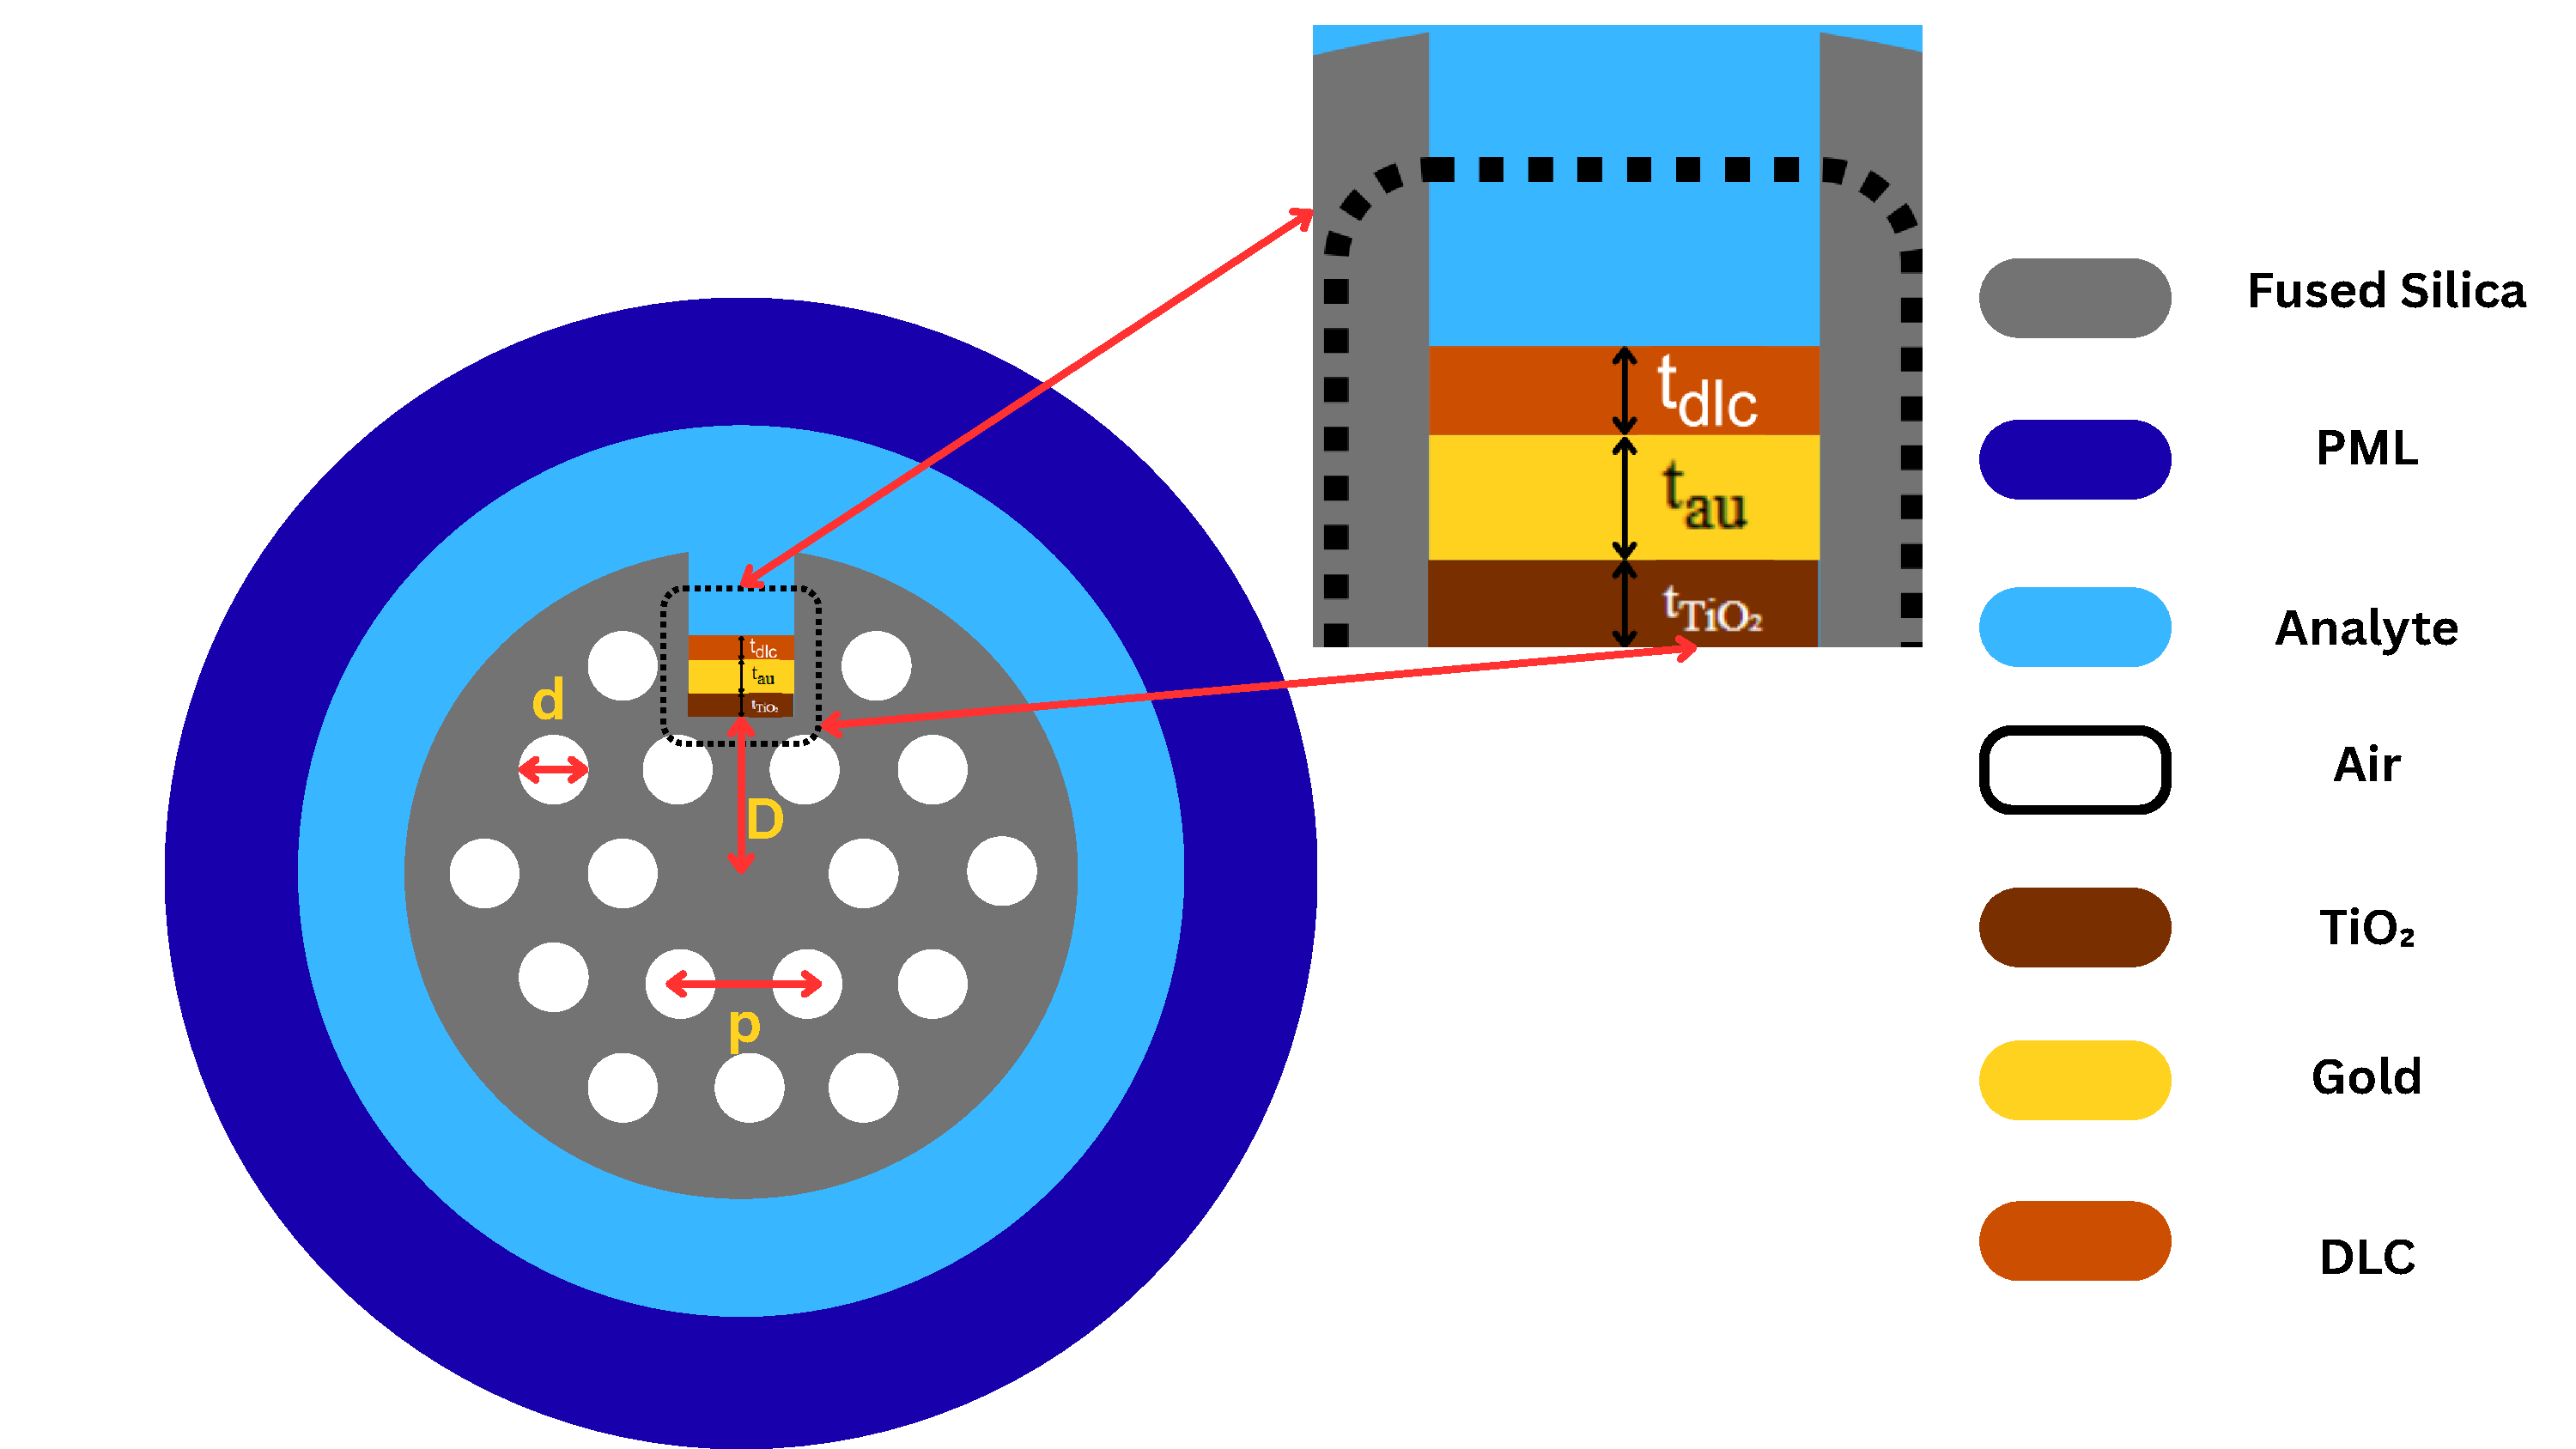
\includegraphics[width=0.75\textwidth]{2D_DES_FINAL_SO.pdf}
    
    \vspace{-1mm}
    {\small (b)}
    
    \caption{(a) Schematic 3-D model. (b) Cross-sectional illustration of the proposed TiO$_2$--Au--DLC coated slotted PCF-SPR sensor.}
    \label{fig:proposed_structure}
\end{figure}

\subsection{\textbf{Numerical Modelling}}

The numerical investigation of the proposed TiO$_2$-Au-DLC coated slotted PCF-SPR sensor is carried out using the finite element method (FEM) in COMSOL Multiphysics 5.6. A circular perfectly matched layer (PML) is applied around the computational region to absorb the outgoing radiation and to reduce unwanted reflection from the outer boundary. The modal analysis is performed in the wavelength interrogation scheme by solving the eigenmode problem of the proposed structure. The analyte refractive index is varied from 1.33 to 1.41 to evaluate the sensing response of the sensor.

In the simulation model, fused silica is used as the background material of the PCF structure. The wavelength-dependent refractive index of fused silica is calculated using the Sellmeier equation \cite{ashrafian2025highly}:

\begin{equation}
n_{\mathrm{SiO_2}}(\lambda)=
\sqrt{
1+\frac{B_1\lambda^2}{\lambda^2-C_1}
+\frac{B_2\lambda^2}{\lambda^2-C_2}
+\frac{B_3\lambda^2}{\lambda^2-C_3}
}
\label{eq:sellmeier_silica}
\end{equation}

where $\lambda$ is the operating wavelength in micrometers. The Sellmeier coefficients for fused silica are selected as $B_1=0.6961663$, $B_2=0.4079426$, $B_3=0.8974794$, $C_1=0.004679148~\mu\mathrm{m}^2$, $C_2=0.0135120631~\mu\mathrm{m}^2$, and $C_3=97.9340025~\mu\mathrm{m}^2$.

Gold is used as the main plasmonic material due to its stable SPR response and strong interaction with the evanescent field. The wavelength-dependent dielectric constant of gold is described by the Drude-Lorentz model \cite{ashrafian2025highly}:

\begin{equation}
\varepsilon_{\mathrm{Au}}(\omega)=
\varepsilon_{\infty}
-\frac{\omega_D^2}{\omega(\omega+i\gamma_D)}
-\frac{\Delta\varepsilon \Omega_L^2}
{(\omega^2-\Omega_L^2)+i\Gamma_L\omega}
\label{eq:gold_drude_lorentz}
\end{equation}

where $\varepsilon_{\infty}$ is the high-frequency dielectric constant, $\omega_D$ is the plasma frequency, $\gamma_D$ is the damping frequency, $\Delta\varepsilon$ is the weighting factor, $\Omega_L$ is the Lorentz oscillator strength, and $\Gamma_L$ is the spectral width of the Lorentz oscillator. The corresponding parameters are taken as $\varepsilon_{\infty}=5.9673$, $\omega_D/2\pi=2113.6$ THz, $\gamma_D/2\pi=15.92$ THz, $\Delta\varepsilon=1.09$, $\Omega_L/2\pi=650.07$ THz, and $\Gamma_L/2\pi=104.86$ THz.

The complex refractive index of gold is obtained from its complex dielectric function as follows:

\begin{equation}
\varepsilon_{\mathrm{Au}}(\omega)=\varepsilon_1(\omega)+j\varepsilon_2(\omega)
\label{eq:gold_complex_eps}
\end{equation}

\begin{equation}
\varepsilon_1=n^2-k^2
\label{eq:eps1}
\end{equation}

\begin{equation}
\varepsilon_2=2nk
\label{eq:eps2}
\end{equation}

\begin{equation}
n_{\mathrm{Au}}=
\sqrt{\frac{\varepsilon_1+\sqrt{\varepsilon_1^2+\varepsilon_2^2}}{2}}
\label{eq:gold_n}
\end{equation}

\begin{equation}
k_{\mathrm{Au}}=
\frac{\varepsilon_2}{2n_{\mathrm{Au}}}
\label{eq:gold_k}
\end{equation}

where $n_{\mathrm{Au}}$ and $k_{\mathrm{Au}}$ represent the real refractive index and extinction coefficient of gold, respectively \cite{maier2007plasmonics}.

A TiO$_2$ layer is introduced between the fused silica and gold layer to improve the coupling condition and to support stronger excitation of the surface plasmon polariton mode. The refractive index of TiO$_2$ is calculated using the following dispersion relation \cite{ashrafian2025highly}:

\begin{equation}
n_{\mathrm{TiO_2}}(\lambda)=
\sqrt{
5.913+\frac{0.2441}{\lambda^2-0.0803}
}
\label{eq:tio2_ri}
\end{equation}

where $\lambda$ is expressed in micrometers.

In this work, a DLC layer is added over the plasmonic region to improve the interaction between the evanescent field and the surrounding analyte medium. The wavelength-dependent refractive index of DLC is expressed as \cite{erdogan2025diamond}:

\begin{equation}
n_{\mathrm{DLC}}(\lambda)=
\sqrt{
A_0+\frac{A_1\lambda^2}{\lambda^2-A_2}
}
\label{eq:dlc_ri}
\end{equation}

where $A_0$, $A_1$, and $A_2$ are the dispersion coefficients of DLC. The values of these coefficients should be selected according to the experimentally reported DLC thin-film data used in the simulation.

The confinement loss is evaluated from the imaginary part of the effective refractive index of the fundamental core-guided mode. It is calculated as \cite{zhang2025highly}:

\begin{equation}
\alpha_{\mathrm{loss}}(\mathrm{dB/cm})=
8.686\times\frac{2\pi}{\lambda}
\times \mathrm{Im}(n_{\mathrm{eff}})\times 10^4
\label{eq:confinement_loss}
\end{equation}

where $\lambda$ is the operating wavelength in micrometers and $\mathrm{Im}(n_{\mathrm{eff}})$ is the imaginary part of the effective refractive index. A higher confinement loss at a particular wavelength indicates stronger coupling between the core-guided mode and the SPP mode. Therefore, the resonance wavelength is identified from the peak position of the confinement loss spectrum.

\subsection{\textbf{Performance Indicating Parameters}}

The sensing performance of the proposed PCF-SPR sensor is evaluated using wavelength sensitivity, amplitude sensitivity, full width at half maximum, figure of merit, and resolution. In wavelength interrogation, the shift of the resonance wavelength due to a change in analyte refractive index is used to calculate the wavelength sensitivity \cite{zhang2025highly}:
\begin{figure}[!t]
    \centering
    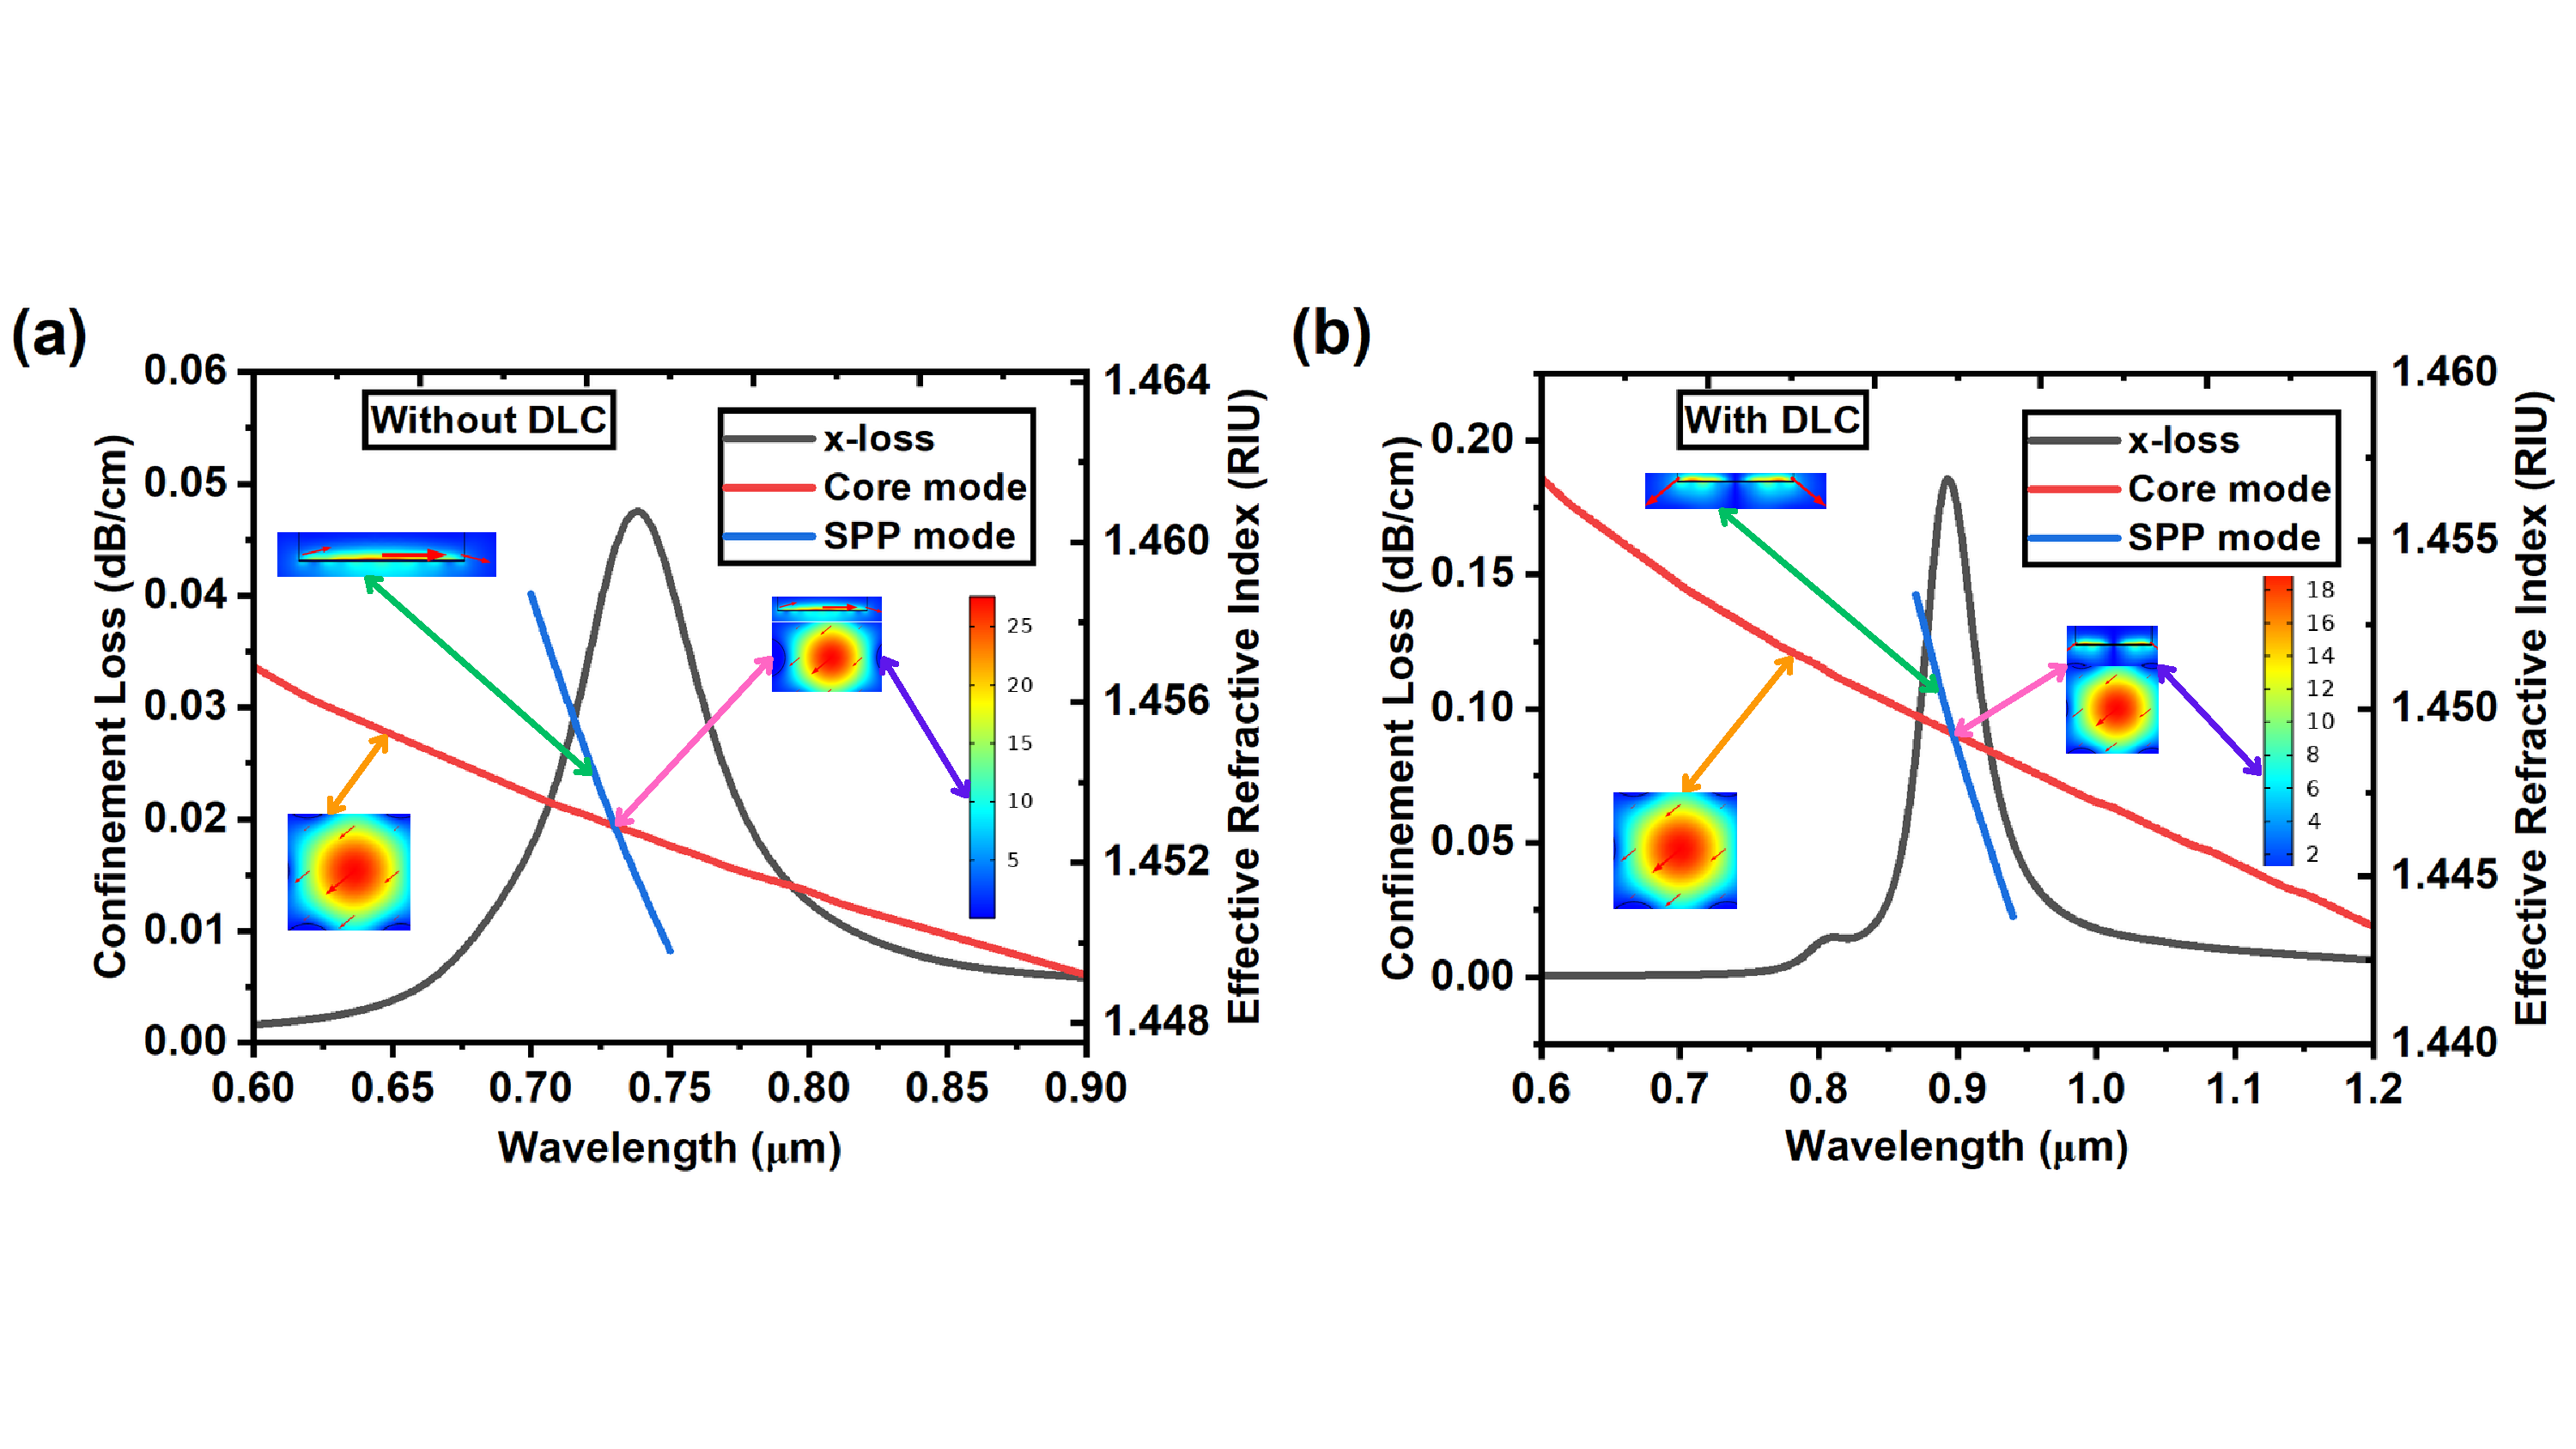
\includegraphics[
        width=1\textwidth,
        trim=0.4cm 6.7cm 0.4cm 5.2cm,
        clip
    ]{Phase_Soumik01.pdf}
    \vspace{-2mm}
    \caption{Phase-matching characteristics of the proposed TiO$_2$--Au--DLC coated slotted PCF-SPR sensor: (a) with DLC coating and (b) without DLC coating.}
    \label{fig:phase_matching}
\end{figure}

\begin{equation}
S_{\lambda}(\mathrm{nm/RIU})=
\frac{\Delta\lambda_{\mathrm{peak}}}{\Delta n_a}
\label{eq:wavelength_sensitivity}
\end{equation}

where $\Delta\lambda_{\mathrm{peak}}$ represents the shift of the resonance wavelength and $\Delta n_a$ denotes the change in analyte refractive index.

The amplitude interrogation method is used to evaluate how strongly the confinement loss changes with the analyte refractive index. In this method, the amplitude sensitivity is calculated from the loss variation at a fixed wavelength. It is expressed as \cite{ashrafian2025highly}:

\begin{equation}
S_A(\lambda)\,[\mathrm{RIU}^{-1}]
=
-\frac{1}{\alpha(\lambda,n_a)}
\frac{\partial \alpha(\lambda,n_a)}{\partial n_a}
\label{eq:amplitude_sensitivity}
\end{equation}

where $\alpha(\lambda,n_a)$ represents the confinement loss of the fundamental core mode at wavelength $\lambda$ and analyte refractive index $n_a$. The term $\partial\alpha(\lambda,n_a)/\partial n_a$ indicates the change in confinement loss due to the change in analyte RI. In this work, the negative sign is kept in the equation, and the amplitude sensitivity values are reported with negative signs.

The detection resolution indicates the smallest RI change that can be detected by the sensor. A lower resolution value means that the sensor can identify a smaller change in the analyte refractive index. The resolution is calculated as \cite{ashrafian2025highly}:

\begin{equation}
R\,[\mathrm{RIU}]
=
\frac{\Delta n_a \times \Delta\lambda_{\min}}
{\Delta\lambda_{\mathrm{peak}}}
\label{eq:resolution}
\end{equation}

where $\Delta n_a$ is the change in analyte refractive index, $\Delta\lambda_{\mathrm{peak}}$ is the resonance wavelength shift between two adjacent RI values, and $\Delta\lambda_{\min}$ is the minimum wavelength resolution of the optical spectrum analyzer. In this work, $\Delta\lambda_{\min}$ is considered as 0.1 nm for calculating the sensor resolution.

The figure of merit (FOM) is used to describe the overall quality of the resonance peak. It depends on both the wavelength sensitivity and the sharpness of the resonance curve. The FOM is defined as \cite{ashrafian2025highly}:

\begin{equation}
\mathrm{FOM}\,[\mathrm{RIU}^{-1}]
=
\frac{S_{\lambda}}{\mathrm{FWHM}}
\label{eq:fom}
\end{equation}

where $S_{\lambda}$ is the wavelength sensitivity and FWHM is the full width at half maximum of the resonance loss peak. A higher $S_{\lambda}$ and a smaller FWHM produce a larger FOM, which indicates a sharper and more reliable sensing response.

where $\Delta\lambda_{\mathrm{min}}$ is the minimum wavelength resolution of the optical spectrum analyzer. In this study, the proposed sensor response is analyzed over the analyte RI range of 1.33-1.41, and the influence of DLC coating is investigated by comparing the sensing parameters with and without the DLC layer.




\subsection{\textbf{{Resonance and Phase-Matching Behavior}}}

The resonance and phase-matching behavior of the proposed TiO$_2$-Au-coated PCF-SPR sensor with and without DLC is illustrated in Fig.~\ref{fig:phase_matching}. This analysis is carried out to clarify the coupling mechanism between the core-guided mode and the surface plasmon polariton (SPP) mode. As shown in Fig.~\ref{fig:phase_matching}(a), the sensor without DLC exhibits a resonance peak near 0.74~$\mu$m. At this wavelength, the effective refractive index of the core mode becomes close to that of the SPP mode, which confirms the phase-matching condition. As a result, part of the optical energy is transferred from the core mode to the plasmonic mode, producing a confinement loss peak.After adding the DLC layer, the resonance peak shifts toward the longer wavelength region, as presented in Fig.~\ref{fig:phase_matching}(b). A stronger and sharper loss peak is observed around 0.90~$\mu$m, indicating enhanced coupling between the core-guided mode and the SPP mode. This improvement occurs because the DLC layer modifies the multilayer sensing interface and increases the interaction between the guided field and the plasmonic surface. Therefore, the DLC layer not only shifts the resonance peak toward a longer wavelength but also strengthens the coupling between the core-guided mode and the SPP mode, leading to improved sensing performance.


\subsection{\textbf{Parametric Optimization of the Proposed Sensor}}

The sensing performance of the proposed PCF-SPR sensor is strongly affected by the geometrical parameters and material layer thicknesses. Therefore, a one-parameter-at-a-time optimization is carried out by varying the air-hole
\begin{figure}[!t]
\centering
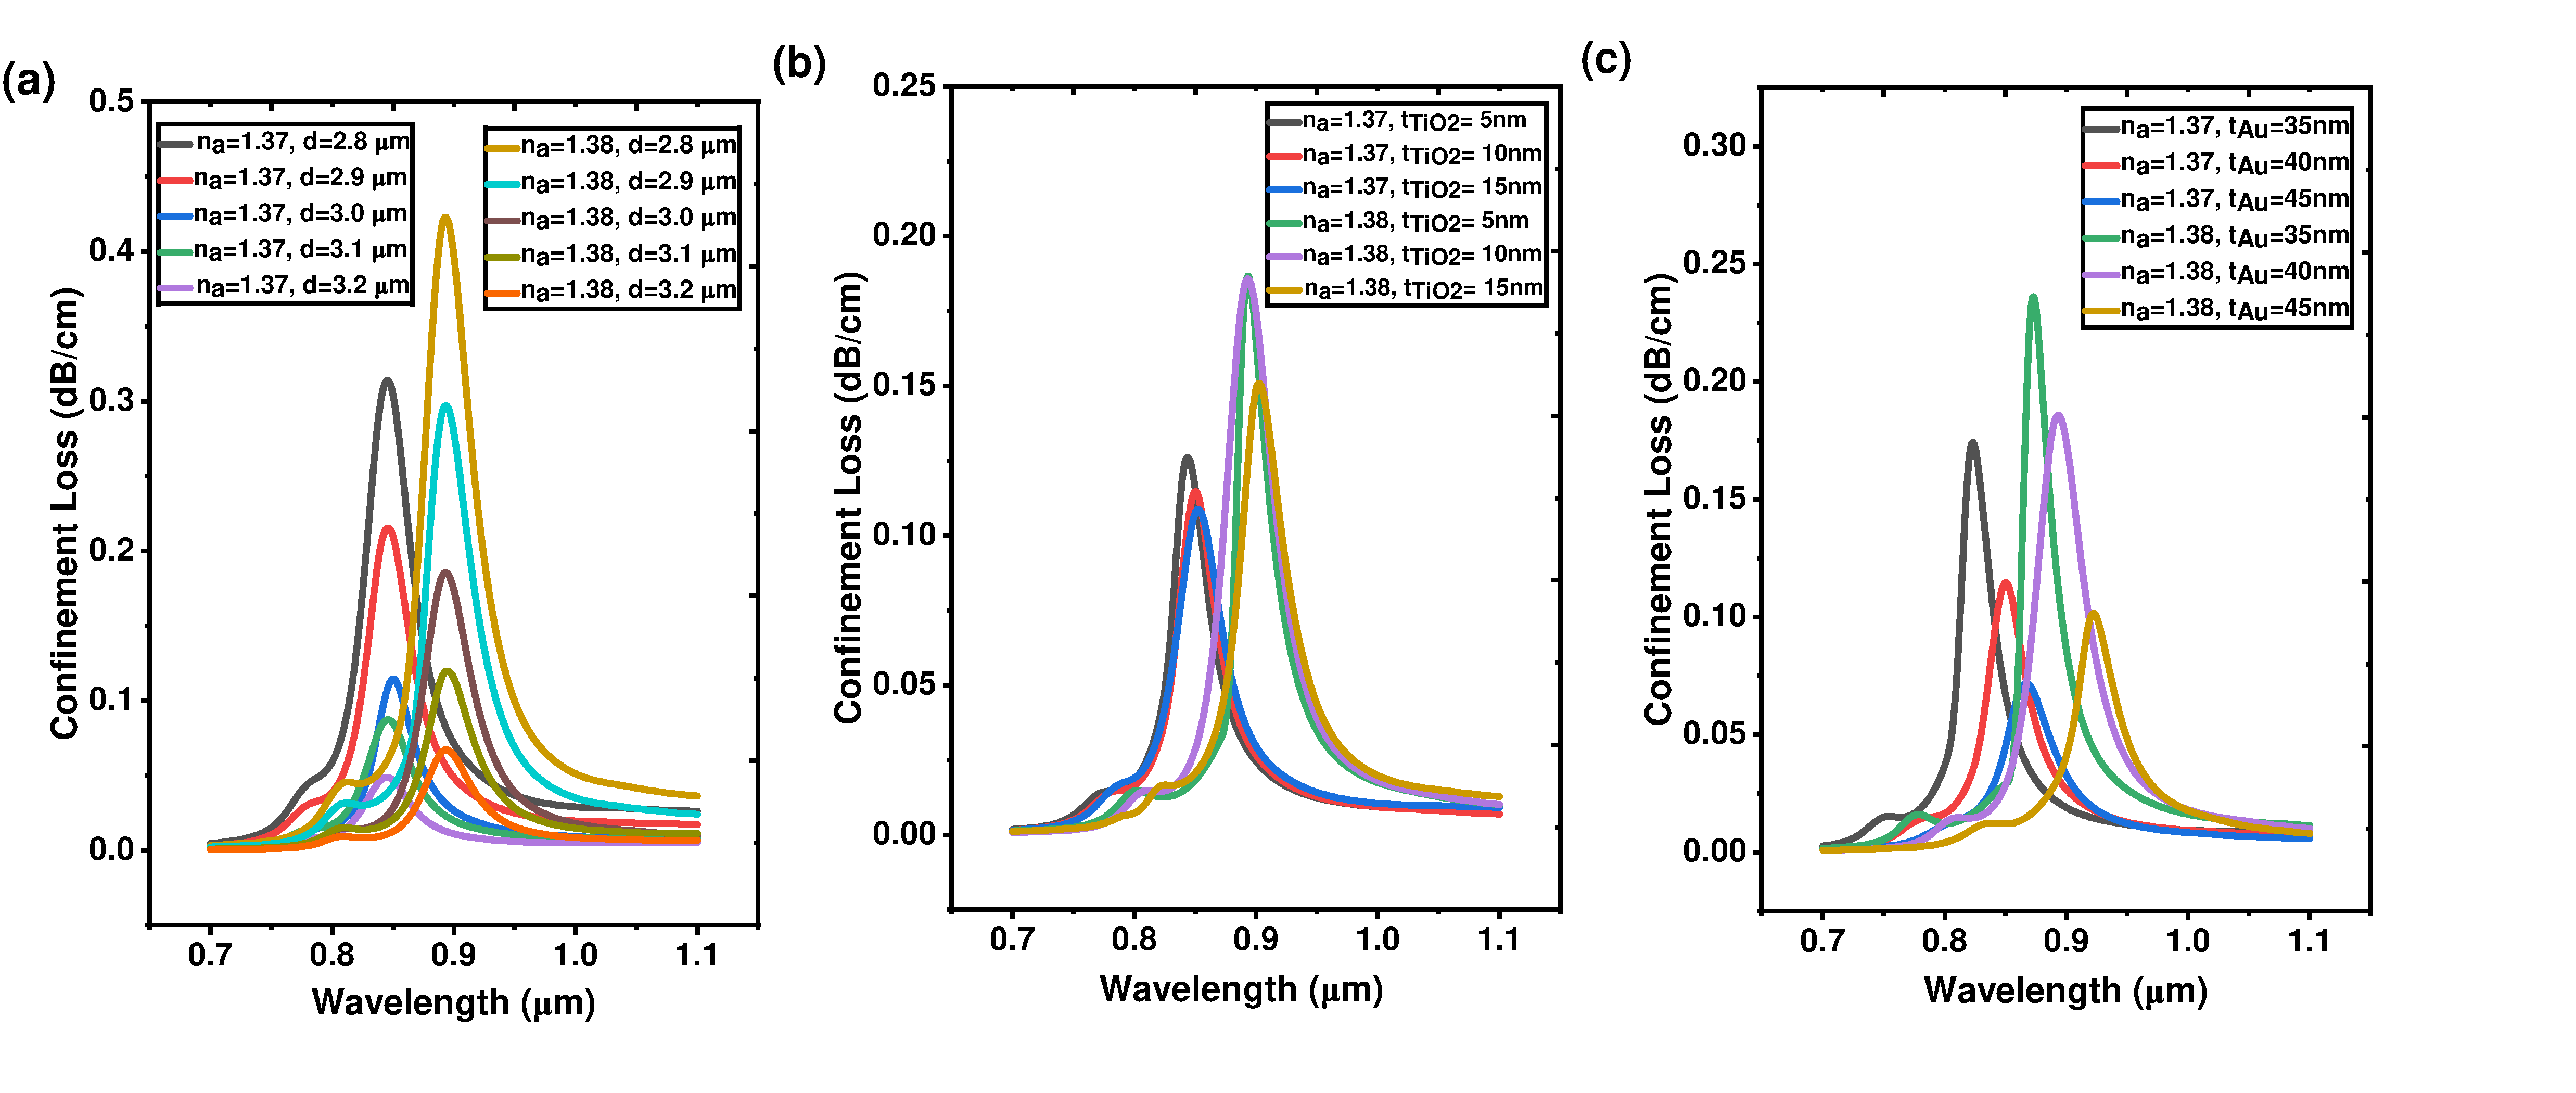
\includegraphics[width=1\textwidth]{D,TIO2,AU(CL)(V-1).pdf}
\caption{Variation of confinement loss with the change in (a) air-hole diameter, (b) TiO$_2$ layer thickness, and (c) Au layer thickness for analyte RI values of 1.37 and 1.38.}
\label{fig:optimization_curves}
\end{figure}
\begin{figure}[!t]
\centering
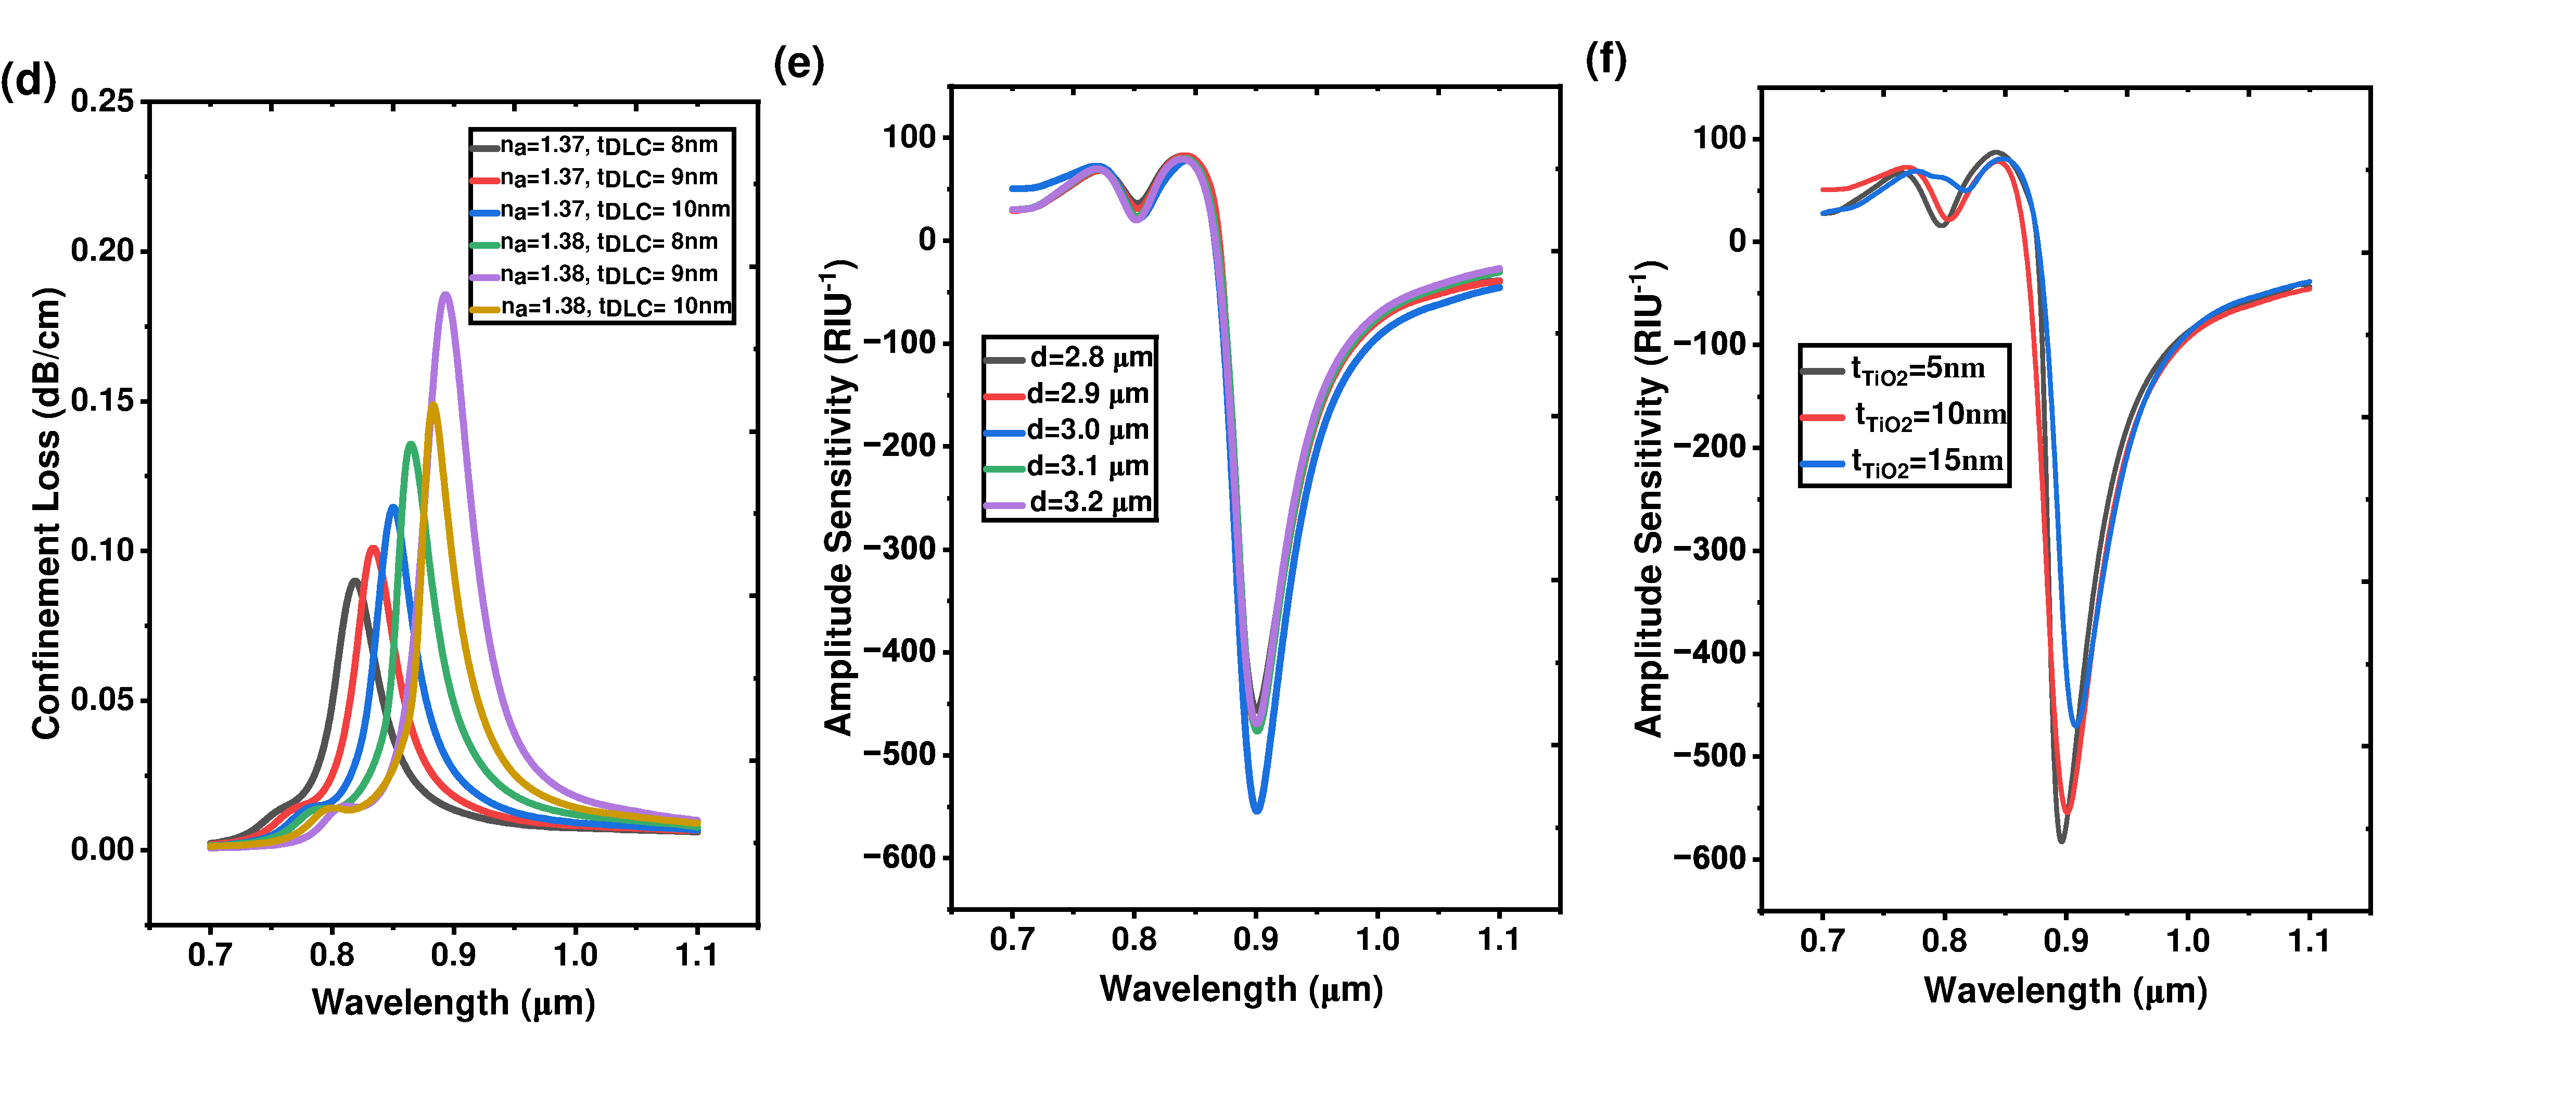
\includegraphics[width=1\textwidth]{CL1,AS2-COM.pdf}
\caption{Variation of (d) confinement loss with DLC layer thickness, and amplitude sensitivity with (e) air-hole diameter and (f) TiO$_2$ layer thickness for analyte RI values of 1.37 and 1.38.}
\label{fig:optimization_d_e_f}
\end{figure}
\begin{figure}[!t]
\centering
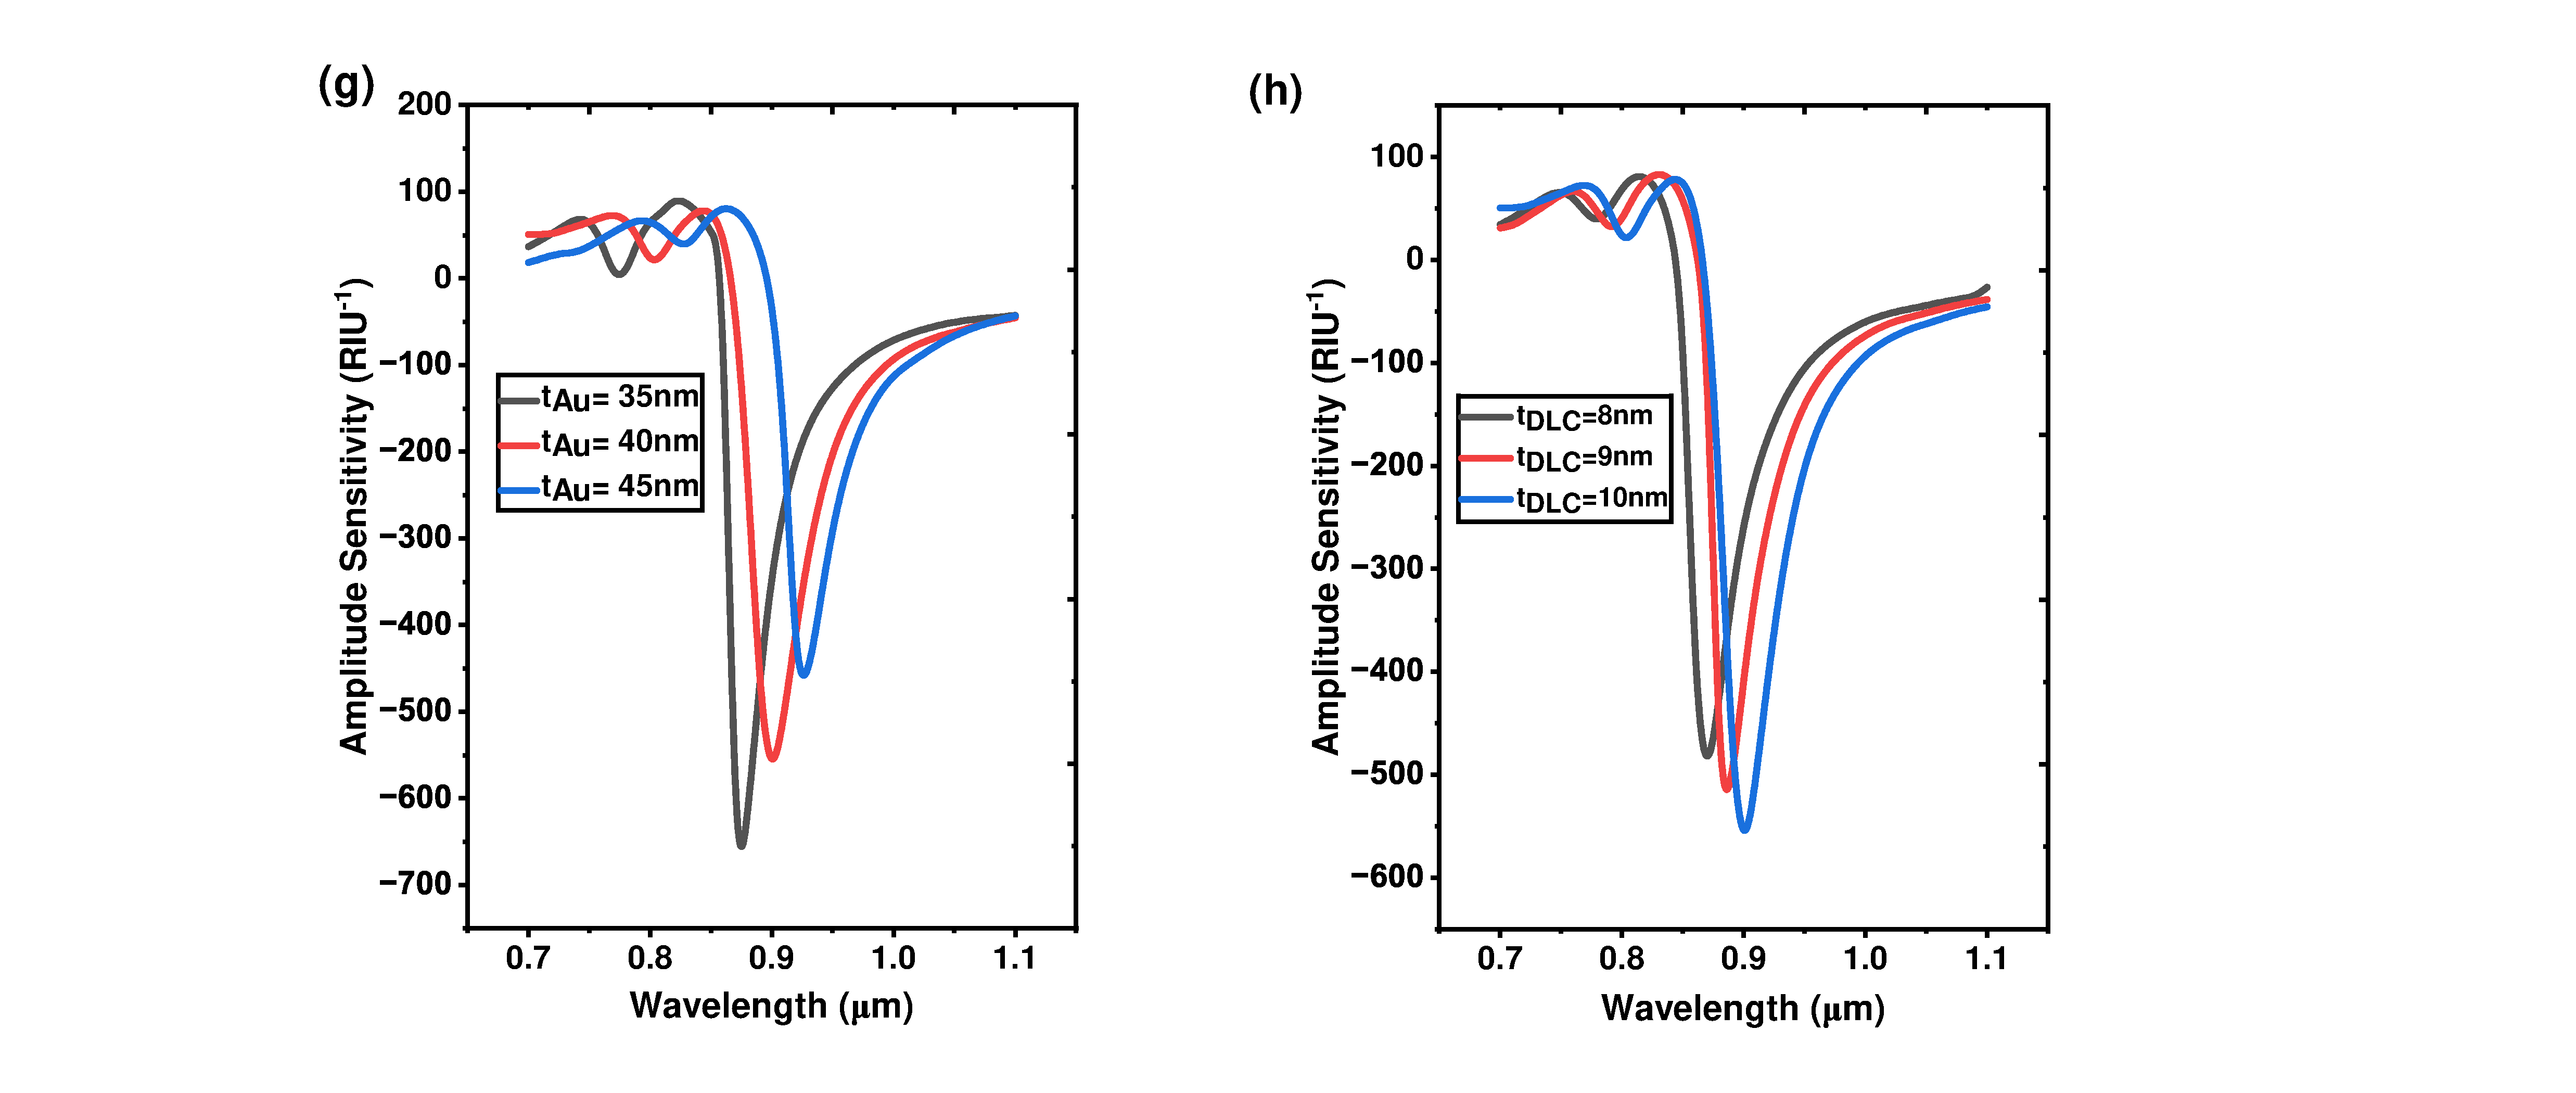
\includegraphics[width=1\textwidth]{final amp-2.pdf}
\caption{Variation of amplitude sensitivity with the change in (g) Au layer thickness and (h) DLC layer thickness for analyte RI values of 1.37 and 1.38.}
\label{fig:optimization_g_h}
\end{figure}
 diameter, TiO$_2$ thickness, Au thickness, and DLC thickness while keeping the other parameters fixed. For each case, the resonance shift, confinement loss, and amplitude sensitivity are analyzed for analyte RI values of 1.37 and 1.38, as shown in Figs.~\ref{fig:optimization_curves}-\ref{fig:optimization_g_h}. The corresponding resonance wavelengths and wavelength sensitivities are listed in Table~\ref{tab:optimization_results}.The final optimized values are not chosen only from the maximum wavelength sensitivity. Instead, they are selected based on a balanced combination of wavelength sensitivity, amplitude sensitivity, and confinement loss. Thus, the selected parameters provide high resonance shift, comparatively strong amplitude response, and clear confinement loss peaks with acceptable loss magnitude.

\subsubsection{\textbf{Optimization of TiO$_2$ Layer Thickness}}
The effect of TiO$_2$ layer thickness on the confinement loss response is shown in Fig.~\ref{fig:optimization_curves}(b), while the corresponding amplitude sensitivity variation is presented in Fig.~\ref{fig:optimization_d_e_f}(f).The thickness of the TiO$_2$ layer is varied as 5 nm, 10 nm, and 15 nm to find a suitable coupling condition for the proposed sensor. From Table~\ref{tab:optimization_results}, the 5 nm TiO$_2$ layer shows higher wavelength sensitivity and amplitude sensitivity. However, this thinner TiO$_2$ layer also produces a higher peak confinement loss, which indicates stronger attenuation of the guided mode. Therefore, although the sensitivity is high, the loss response becomes comparatively large.When the TiO$_2$ thickness is increased to 15 nm, the peak confinement loss decreases. However, the amplitude sensitivity also decreases, which means that the interaction between the evanescent field and the analyte region becomes weaker. Thus, a thicker TiO$_2$ layer can reduce the loss, but it may also reduce the sensing response.Considering wavelength sensitivity, amplitude sensitivity, and peak confinement loss together, the 10 nm TiO$_2$ layer is selected as the optimized thickness. It provides a balanced condition where the confinement loss is not excessively high and the amplitude sensitivity remains acceptable. Therefore, $t_{\mathrm{TiO_2}} = 10~\mathrm{nm}$ is chosen for the final sensor design to maintain a stable and reliable SPR response.
\begin{table}[!t]
\centering
\caption{Optimized Design Parameters of the Proposed Sensor}
\label{tab:optimization_results}
\renewcommand{\arraystretch}{1.5}
\setlength{\tabcolsep}{2.5pt}
\scriptsize

\resizebox{\textwidth}{!}{
\begin{tabular}{|c|c|c|c|c|c|c|c|}
\hline
\textbf{Parameter} 
& \textbf{Value}
& \multicolumn{2}{c|}{\textbf{$\lambda_{\mathrm{peak}}$ ($\mu$m)}} 
& \multicolumn{2}{c|}{\textbf{Peak CL (dB/cm)}} 
& \textbf{$S_{\lambda}$} 
& \textbf{$S_A$} \\
\cline{3-6}
& 
& \textbf{$n_a=1.37$} 
& \textbf{$n_a=1.38$} 
& \textbf{$n_a=1.37$} 
& \textbf{$n_a=1.38$} 
& \textbf{(nm/RIU)} 
& \textbf{(RIU$^{-1}$)} \\
\hline

\multirow{3}{*}{$t_{\mathrm{TiO_2}}$ (nm)}
& 5  & 0.84 & 0.89 & 0.1370 & 0.2146 & 5000 & -614.85 \\
& \textbf{10} & 0.85 & 0.89 & 0.1256 & 0.1939 & 4000 & -583.55 \\
& 15 & 0.85 & 0.90 & 0.1148 & 0.1621 & 5000 & -485.07 \\
\hline

\multirow{3}{*}{$t_{\mathrm{Au}}$ (nm)}
& 35 & 0.82 & 0.87 & 0.1977 & 0.2809 & 5000 & -723.30 \\
& \textbf{40} & 0.85 & 0.89 & 0.1256 & 0.1939 & 4000 & -583.55 \\
& 45 & 0.87 & 0.92 & 0.0743 & 0.1114 & 5000 & -469.62 \\
\hline

\multirow{3}{*}{$t_{\mathrm{DLC}}$ (nm)}
& 8  & 0.82 & 0.86 & 0.0959 & 0.1438 & 4000 & -511.56 \\
& 9  & 0.83 & 0.88 & 0.1067 & 0.1689 & 5000 & -537.94 \\
& \textbf{10} & 0.85 & 0.89 & 0.1256 & 0.1939 & 4000 & -583.55 \\
\hline

\multirow{5}{*}{$d$ ($\mu$m)}
& 2.8 & 0.85 & 0.89 & 0.3182 & 0.4418 & 4000 & -479.08 \\
& 2.9 & 0.85 & 0.89 & 0.2197 & 0.3109 & 4000 & -497.33 \\
& \textbf{3.0} & 0.85 & 0.89 & 0.1256 & 0.1939 & 4000 & -583.55 \\
& 3.1 & 0.85 & 0.89 & 0.0894 & 0.1234 & 4000 & -503.97 \\
& 3.2 & 0.84 & 0.89 & 0.0499 & 0.0697 & 5000 & -494.99 \\
\hline



\end{tabular}
}
\end{table}
Although the maximum wavelength sensitivity is slightly higher for 5 nm and 15 nm, only sensitivity is not considered as the single optimization criterion. A stable resonance peak, clear spectral shift, and balanced confinement loss response are also important for reliable sensing. Therefore, $t_{\mathrm{TiO_2}} = 10~\mathrm{nm}$ is selected as the optimized TiO$_2$ thickness.

\subsubsection{\textbf{{Optimization of Au Layer Thickness}}}
The effect of Au layer thickness on the confinement loss response is illustrated in Fig.~\ref{fig:optimization_curves}(c), and the corresponding amplitude sensitivity variation is shown in Fig.~\ref{fig:optimization_g_h}(g).
The thickness of the Au layer is varied as 35 nm, 40 nm, and 45 nm to find a suitable plasmonic condition for the proposed sensor. From Table~\ref{tab:optimization_results}, the 35 nm Au layer shows higher wavelength sensitivity and amplitude sensitivity. However, this thinner Au layer also produces a higher peak confinement loss, which indicates stronger attenuation of the guided mode. Therefore, although the sensitivity is high, the loss response becomes comparatively large.When the Au thickness is increased to 45 nm, the peak confinement loss decreases. However, the amplitude sensitivity also decreases, which means that the interaction between the evanescent field and the analyte region becomes weaker. Thus, a thicker Au layer can reduce the sensing response even though the loss becomes lower.Considering these three factors together, the 40 nm Au layer is selected as the optimized thickness. It provides a balanced condition among wavelength sensitivity, amplitude sensitivity, and peak confinement loss. Therefore, $t_{\mathrm{Au}} = 40~\mathrm{nm}$ is chosen for the final sensor design to maintain a stable and reliable SPR response.

\subsubsection{\textbf{{Optimization of DLC Layer Thickness}}}
The effect of DLC layer thickness on the confinement loss response is shown in Fig.~\ref{fig:optimization_d_e_f}(d), while the corresponding amplitude sensitivity response is presented in Fig.~\ref{fig:optimization_g_h}(h).
The thickness of the DLC layer is varied as 8 nm, 9 nm, and 10 nm to find a suitable coating condition for improving the sensing response of the proposed sensor. From Table~\ref{tab:optimization_results}, the 8 nm DLC layer shows lower wavelength sensitivity and lower amplitude sensitivity. It also produces a lower peak confinement loss compared with the 10 nm case. This indicates that the interaction between the evanescent field and the analyte region is comparatively weak for the 8 nm DLC layer.For the 9 nm DLC layer, the wavelength sensitivity increases to 5000 nm/RIU. However, the amplitude sensitivity remains lower than that of the 10 nm DLC layer. Therefore, although the resonance wavelength shift is higher for 9 nm, the amplitude response of the sensor is not the strongest.When the DLC thickness is increased to 10 nm, the wavelength sensitivity becomes slightly lower than the 9 nm case. However, the amplitude sensitivity becomes higher, and the peak confinement loss remains within an acceptable range. This indicates stronger interaction between the guided mode, plasmonic layer, and analyte region. Considering wavelength sensitivity, amplitude sensitivity, and peak confinement loss together, the 10 nm DLC layer is selected as the optimized thickness. Therefore, $t_{\mathrm{DLC}} = 10~\mathrm{nm}$ is chosen for the final sensor design.

\subsubsection{\textbf{{Optimization of Air-Hole Diameter}}}
The influence of air-hole diameter on the confinement loss response is presented in Fig.~\ref{fig:optimization_curves}(a), and the corresponding amplitude sensitivity variation is shown in Fig.~\ref{fig:optimization_d_e_f}(e). The air-hole diameter, $d$, is varied as $2.8~\mu\mathrm{m}$, $2.9~\mu\mathrm{m}$, $3.0~\mu\mathrm{m}$, $3.1~\mu\mathrm{m}$, and $3.2~\mu\mathrm{m}$ to investigate its effect on the sensing response of the proposed sensor. From Table~\ref{tab:optimization_results}, the diameter values from $2.8~\mu\mathrm{m}$ to $3.1~\mu\mathrm{m}$ provide the same wavelength sensitivity of 4000 nm/RIU, while $d=3.2~\mu\mathrm{m}$ gives a higher wavelength sensitivity of 5000 nm/RIU.However, the optimized value is not selected based on wavelength sensitivity alone. For $d=2.8~\mu\mathrm{m}$ and $d=2.9~\mu\mathrm{m}$, the peak confinement loss is comparatively high, which indicates stronger attenuation of the guided mode. On the other hand, when the diameter is increased to $3.1~\mu\mathrm{m}$ and $3.2~\mu\mathrm{m}$, the peak confinement loss decreases, but the amplitude sensitivity also decreases. This indicates that the interaction between the guided mode and the sensing region becomes weaker for larger air-hole diameters.Among the investigated values, $d=3.0~\mu\mathrm{m}$ provides the highest amplitude sensitivity while maintaining an acceptable peak confinement loss and stable wavelength sensitivity. Although $d=3.2~\mu\mathrm{m}$ shows a higher wavelength sensitivity, its amplitude sensitivity is much lower and the confinement loss response becomes comparatively weak. Therefore, considering wavelength sensitivity, amplitude sensitivity, and peak confinement loss together, $d=3.0~\mu\mathrm{m}$ is selected as the optimized air-hole diameter for the final sensor design.


\section{\textbf{Effect of DLC Layer on Sensing Performance}}

After completing the geometrical optimization of the proposed slotted PCF-SPR sensor, the influence of the diamond-like carbon (DLC) layer is investigated in detail. The main objective of this analysis is to evaluate whether the additional DLC coating can enhance the sensing response compared with the conventional structure without DLC. For this purpose, the optimized sensor is analyzed over the analyte refractive index range of 1.33-1.41 for both cases: with DLC and without DLC. The confinement loss, amplitude sensitivity, wavelength sensitivity, FWHM, FOM, and resolution are compared to clearly demonstrate the performance improvement introduced by the DLC layer.
\begin{figure}[!t]
    \centering
    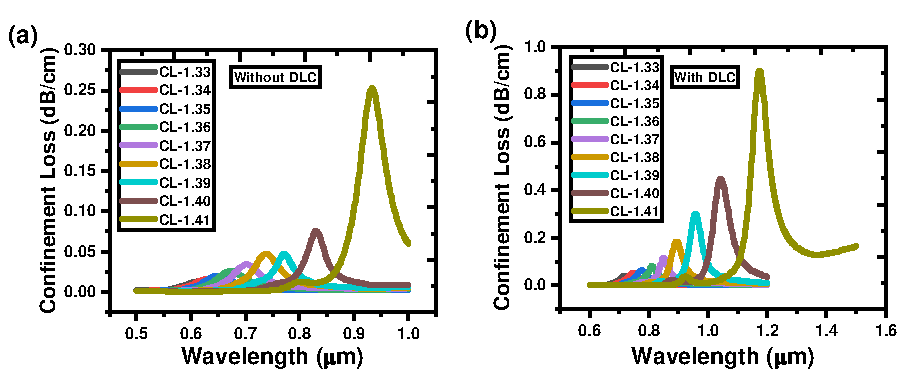
\includegraphics[width=1\textwidth]{CL-(with_without_DLC)-(Soumik).pdf}
    \caption{\normalsize Comparison of confinement loss spectra of the proposed PCF-SPR sensor: (a) without DLC coating and (b) with DLC coating over the analyte RI range of 1.33-1.41.}
    \label{fig:with_without_cl}
\end{figure}
\begin{figure}[!t]
    \centering
    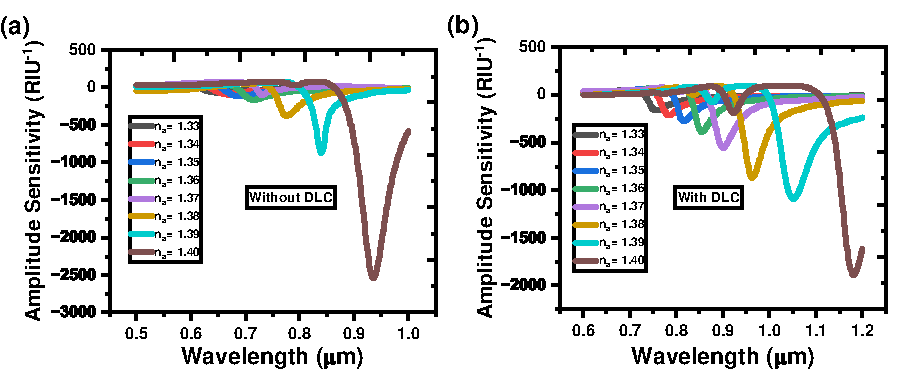
\includegraphics[width=1\textwidth]{Amplitude_sen(1.33-1.41)c.pdf}
    \caption{\normalsize Comparison of amplitude sensitivity response of the proposed PCF-SPR sensor: (a) without DLC coating and (b) with DLC coating over the analyte RI range of 1.33-1.41.}
    \label{fig:with_without_as}
\end{figure}

\subsection{\textbf{Confinement Loss Response With and Without DLC}}

Fig.~\ref{fig:with_without_cl} compares the confinement loss spectra of the proposed sensor without and with the DLC layer for the analyte RI range of 1.33-1.41. In both cases, the resonance peak changes its position when the analyte RI increases. This happens because the change in RI affects the phase-matching condition between the core-guided mode and the SPP mode.Compared with the sensor without DLC, the DLC-coated structure shows a larger resonance wavelength shift for the same RI change. This is important because wavelength sensitivity depends on how much the resonance peak shifts for a given RI variation. Therefore, the improved sensing response mainly comes from the larger peak shift obtained after adding the DLC layer.
The DLC layer also makes the resonance peak more noticeable, which indicates better coupling between the core mode and the SPP mode. As a result, the light interaction with the analyte becomes stronger, and the overall sensing performance of the proposed PCF-SPR sensor is improved.


\subsection{\textbf{Amplitude Sensitivity Response With and Without DLC}}

Fig.~\ref{fig:with_without_as} compares the amplitude sensitivity response of the proposed sensor without and with the DLC layer. The amplitude sensitivity curves show noticeable dips for different analyte RI values, which confirms that the sensor response changes with the variation of refractive index.After adding the DLC layer, the sensitivity dips become deeper and more distinct for most of the investigated RI values, especially in the RI range of 1.33-1.39. This indicates that the DLC coating improves the interaction between the evanescent field, plasmonic layer, and analyte medium. As a result, the sensor becomes more responsive to RI changes in this range.However, for some higher RI values, the structure without DLC may show a deeper amplitude sensitivity dip. Therefore, the performance improvement of the DLC-coated sensor is not claimed only from the maximum amplitude sensitivity value. Rather, the overall improvement is supported by the clearer amplitude response for most RI values, larger resonance wavelength shift, and enhanced wavelength sensitivity after introducing the DLC layer.


\subsection{\textbf{Performance Parameter Analysis}}

The major performance parameters of the proposed sensor without DLC and with DLC coating are compared in Fig.~\ref{fig:performance_comparison} and Table~\ref{tab:performance_matrix}. The comparison includes wavelength sensitivity (WS), amplitude sensitivity (AS), full width at half maximum (FWHM), figure of merit (FOM), and sensor resolution. From the overall trend, it is observed that the DLC-coated structure provides better performance for most of the investigated RI values, especially in the RI range of 1.33-1.39. This improvement is mainly related to the stronger interaction between the guided core mode and the plasmonic surface after adding the DLC layer.
\begin{figure}[!t]
\centering

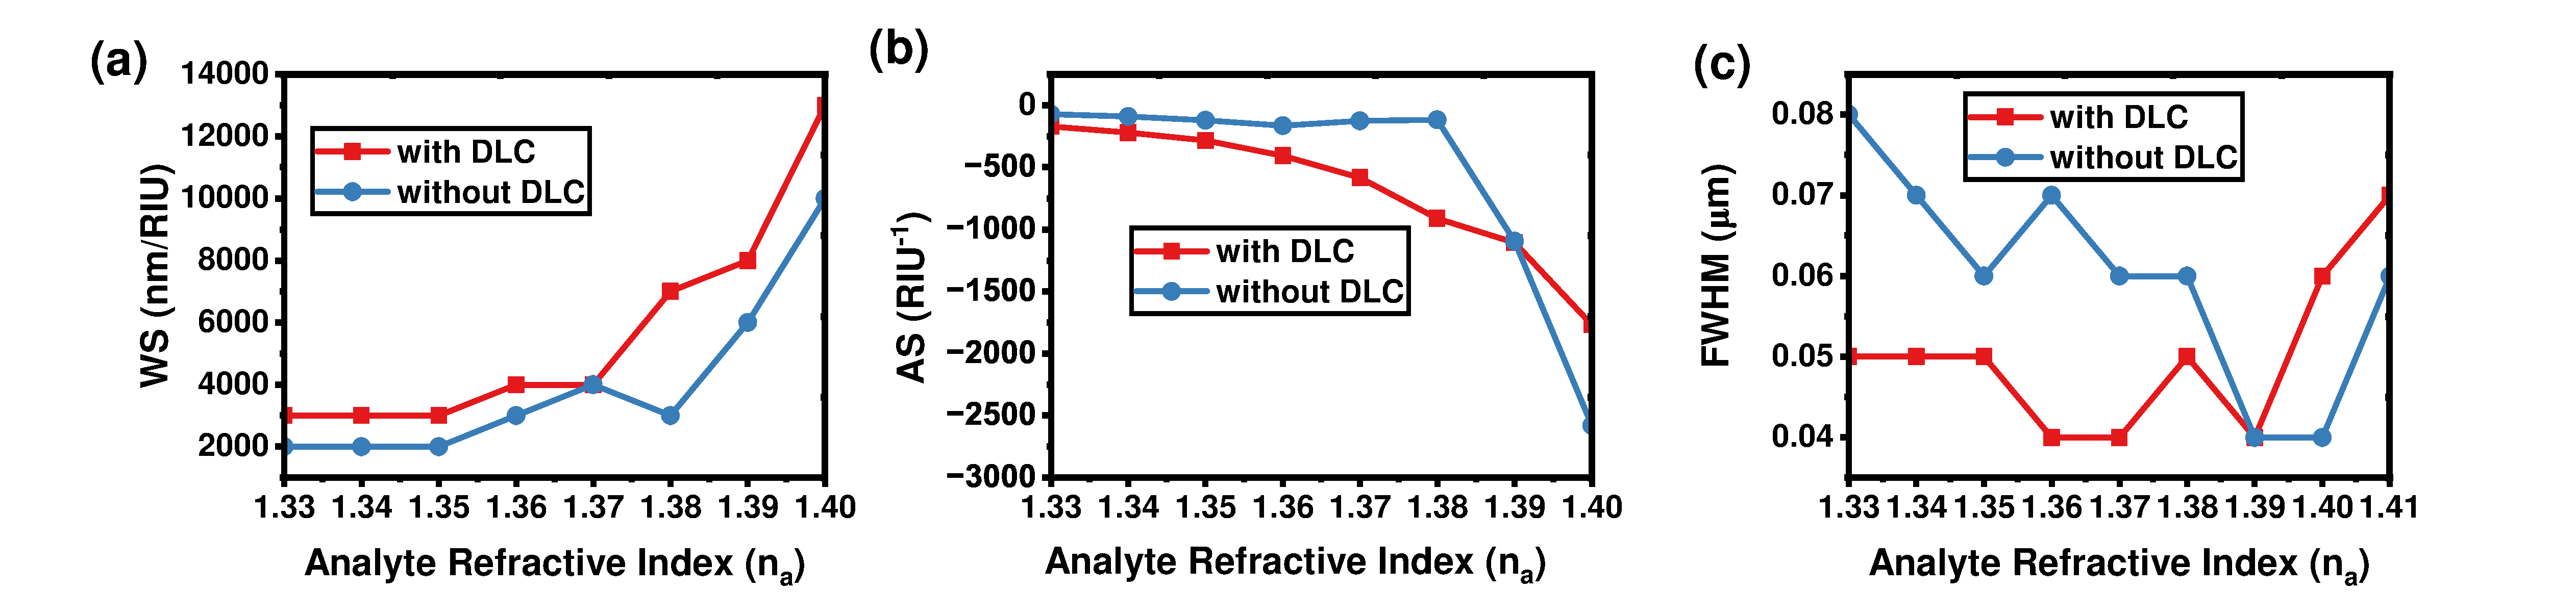
\includegraphics[width=1\textwidth]{WS+AS+FWHM(2).pdf}

\vspace{0.25cm}

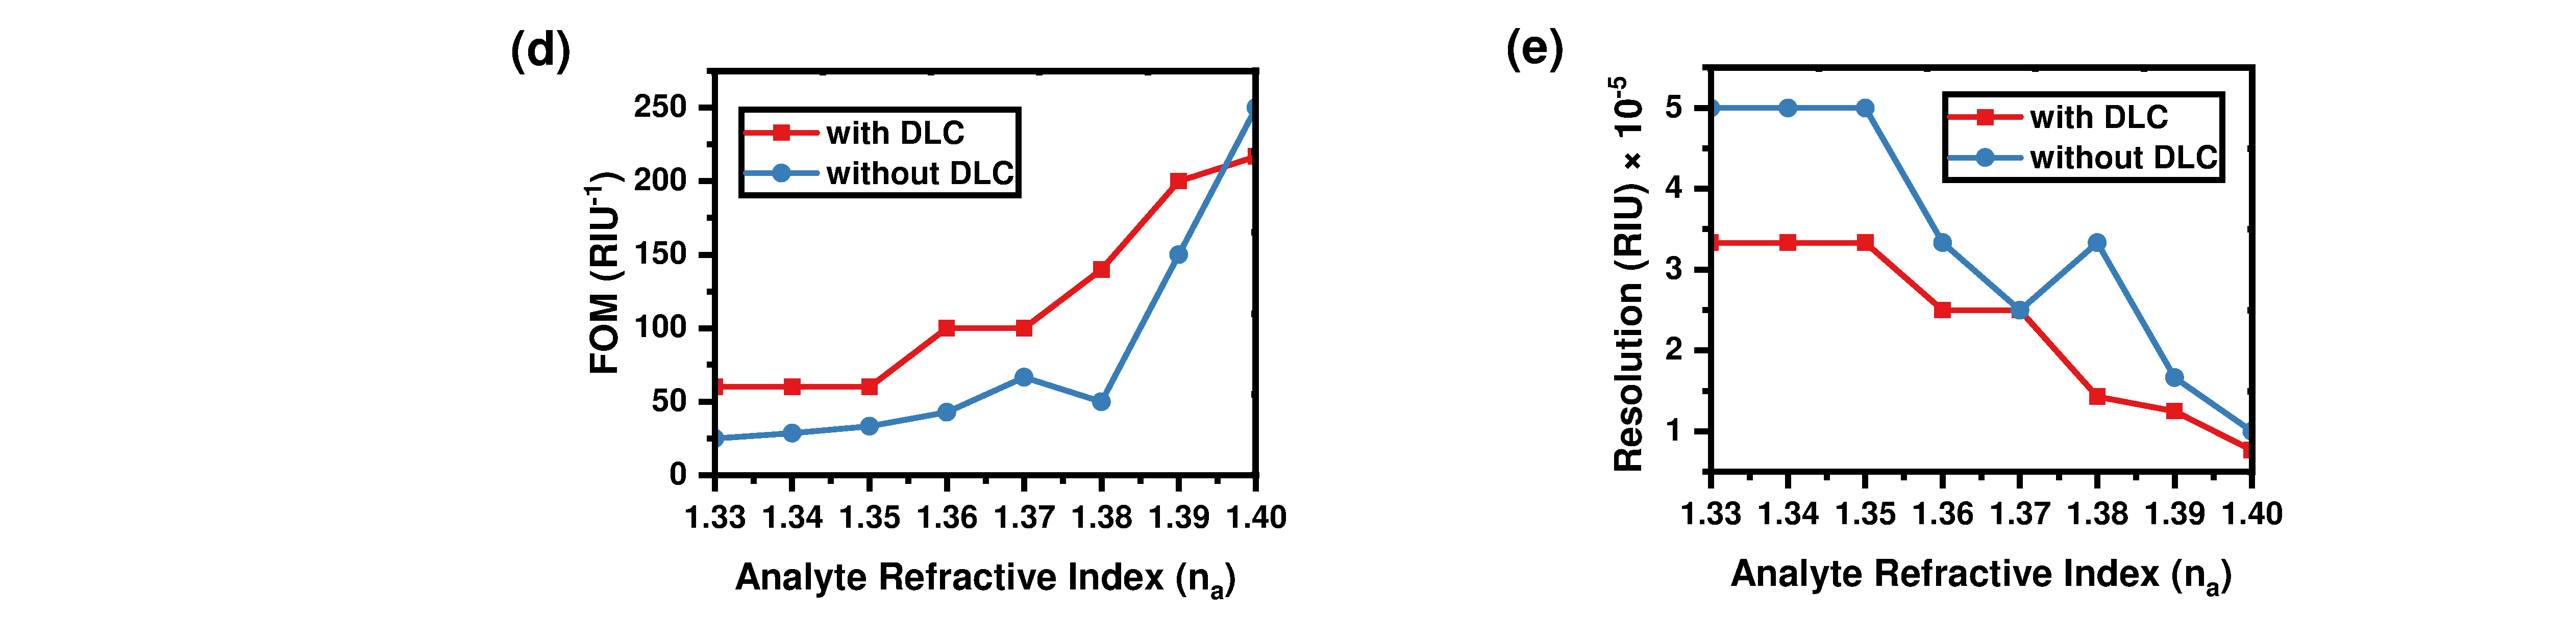
\includegraphics[width=1\textwidth]{FOM+RESOLUTION(2).pdf}

\caption{Comparison of major performance parameters of the proposed sensor without DLC and with DLC coating: (a) wavelength sensitivity, (b) amplitude sensitivity, (c) FWHM, (d) FOM, and (e) resolution.}
\label{fig:performance_comparison}
\end{figure}

\begin{table}[!t]
\centering
\caption{ Performance comparison of the proposed sensor without DLC and with DLC coating.}
\label{tab:performance_matrix}
\normalsize
\setlength{\tabcolsep}{4pt}
\renewcommand{\arraystretch}{1.5}
\resizebox{\textwidth}{!}{
\begin{tabular}{|c|c|c|c|c|c|c|c|c|c|c|}
\hline
\textbf{RI} 
& \multicolumn{2}{c|}{\textbf{WS (nm/RIU)}} 
& \multicolumn{2}{c|}{\textbf{AS (RIU$^{-1}$)}} 
& \multicolumn{2}{c|}{\textbf{FWHM ($\mu$m)}} 
& \multicolumn{2}{c|}{\textbf{FOM (RIU$^{-1}$)}} 
& \multicolumn{2}{c|}{\textbf{Resolution (RIU)}} \\
\cline{2-11}
& \textbf{Without DLC} & \textbf{With DLC}
& \textbf{Without DLC} & \textbf{With DLC}
& \textbf{Without DLC} & \textbf{With DLC}
& \textbf{Without DLC} & \textbf{With DLC}
& \textbf{Without DLC} & \textbf{With DLC} \\
\hline
1.33 & 2000  & 3000  & -71.47  & -170.75  & 0.08 & 0.05 & 25    & 60     & $5.0\times10^{-5}$ & $3.3\times10^{-5}$ \\
1.34 & 2000  & 3000  & -90.91  & -220.98  & 0.07 & 0.05 & 28.57 & 60     & $5.0\times10^{-5}$ & $3.3\times10^{-5}$ \\
1.35 & 2000  & 3000  & -121.26 & -283.75  & 0.06 & 0.05 & 33.33 & 60     & $5.0\times10^{-5}$ & $3.3\times10^{-5}$ \\
1.36 & 3000  & 4000  & -163.78 & -406.46  & 0.07 & 0.04 & 42.86 & 100    & $3.0\times10^{-5}$ & $2.5\times10^{-5}$ \\
1.37 & 4000  & 4000  & -125.62 & -583.55  & 0.06 & 0.04 & 66.67 & 100    & $2.5\times10^{-5}$ & $2.5\times10^{-5}$ \\
1.38 & 3000  & 7000  & -117.40 & -912.15  & 0.06 & 0.05 & 50    & 140    & $3.0\times10^{-5}$ & $1.4\times10^{-5}$ \\
1.39 & 6000  & 8000  & -1094.3 & -1106.6  & 0.04 & 0.04 & 150   & 200    & $1.7\times10^{-5}$ & $1.3\times10^{-5}$ \\
1.40 & 10000 & 13000 & -2580.0 & -1768.4  & 0.04 & 0.06 & 250   & 216.67 & $1.0\times10^{-5}$ & $7.7\times10^{-6}$ \\
\hline
\end{tabular}
}
\end{table}

Fig.~\ref{fig:performance_comparison}(a) shows the wavelength sensitivity response of both structures. From Table~\ref{tab:performance_matrix}, the WS increases from 2000 nm/RIU to 3000 nm/RIU at RI values of 1.33, 1.34, and 1.35 after adding DLC. At RI = 1.38, the WS improves significantly from 3000 nm/RIU without DLC to 7000 nm/RIU with DLC. The highest WS of the DLC-coated sensor is 13000 nm/RIU at RI = 1.40, whereas the sensor without DLC gives 10000 nm/RIU at the same RI. This confirms that the DLC layer increases the resonance wavelength shift caused by analyte RI variation.

The amplitude sensitivity response is presented in Fig.~\ref{fig:performance_comparison}(b). In this work, the AS values are negative because of the mathematical form of the amplitude sensitivity equation. A larger negative value indicates a stronger amplitude response. From Table~\ref{tab:performance_matrix}, the DLC-coated sensor shows improved AS for most RI values. At RI = 1.36, the AS changes from $-163.78$ RIU$^{-1}$ without DLC to $-406.46$ RIU$^{-1}$ with DLC. Similarly, at RI = 1.38, the AS improves from $-117.40$ RIU$^{-1}$ to $-912.15$ RIU$^{-1}$. This stronger negative AS response indicates that the DLC-coated structure is more responsive to small changes in analyte RI.

Fig.~\ref{fig:performance_comparison}(c) shows the FWHM variation. A lower FWHM is preferred because it represents a sharper resonance peak and better detection accuracy. From Table~\ref{tab:performance_matrix}, the DLC-coated sensor gives lower FWHM for most RI values from 1.33 to 1.38. At RI = 1.33, the FWHM decreases from 0.08 $\mu$m without DLC to 0.05 $\mu$m with DLC. At RI = 1.36, it decreases from 0.07 $\mu$m to 0.04 $\mu$m. The narrower resonance peaks obtained after adding DLC help to improve the sensing quality of the proposed sensor.

The FOM response is shown in Fig.~\ref{fig:performance_comparison}(d). Since FOM depends on both WS and FWHM, a higher FOM indicates better overall sensing performance. From Table~\ref{tab:performance_matrix}, the DLC-coated sensor shows higher FOM for most RI values in the range of 1.33--1.39. At RI = 1.36, the FOM increases from 42.86 RIU$^{-1}$ without DLC to 100 RIU$^{-1}$ with DLC. At RI = 1.38, it increases from 50 RIU$^{-1}$ to 140 RIU$^{-1}$. The DLC-coated sensor also reaches a high FOM of 216.67 RIU$^{-1}$ at RI = 1.40.

Fig.~\ref{fig:performance_comparison}(e) presents the resolution of both structures. A lower resolution value is desirable because it means the sensor can detect smaller RI changes. From Table~\ref{tab:performance_matrix}, the DLC-coated sensor provides better resolution for most of the investigated RI values. At RI = 1.33, the resolution improves from $5.0\times10^{-5}$ RIU without DLC to $3.3\times10^{-5}$ RIU with DLC. At RI = 1.38, it improves from $3.0\times10^{-5}$ RIU to $1.4\times10^{-5}$ RIU. The best resolution of the DLC-coated sensor is obtained as $7.7\times10^{-6}$ RIU at RI = 1.40.

A few exceptions are observed at the higher RI region. At RI = 1.40, the sensor without DLC shows a stronger AS value, lower FWHM, and slightly higher FOM than the DLC-coated structure. This may happen because the resonance coupling condition changes at higher analyte RI, and the multilayer interface can slightly broaden the resonance peak. However, considering the full investigated RI range, the DLC-coated sensor improves the performance in most cases. Therefore, the addition of DLC is effective for enhancing the overall sensing response of the proposed PCF-SPR sensor.

\subsection{\textbf{{Comparative Performance Analysis}}}

Table~\ref{tab:comparative_analysis} compares the proposed sensor with selected reported SPR-based sensors that use Au, Au--TiO$_2$, or Au--TiO$_2$-based hybrid coating structures. This comparison is made with similar plasmonic material platforms so that the performance of the proposed DLC-enhanced TiO$_2$-Au-coated sensor can be judged more fairly.

From the table, the reported sensors show maximum wavelength sensitivities from 5000 nm/RIU to 11428.57 nm/RIU. These sensors have been used for biochemical RI sensing, food-quality monitoring, pathogen detection, and biomolecule detection. In comparison, the proposed sensor achieves a higher 
\begin{table}[!t]
\centering
\caption{Comparative analysis of the proposed sensor with selected reported SPR-based sensors.}
\label{tab:comparative_analysis}
\renewcommand{\arraystretch}{2.55}
\setlength{\tabcolsep}{2.2pt}
\footnotesize

\resizebox{\textwidth}{!}{
\begin{tabular}{|c|
>{\RaggedRight\arraybackslash}p{3.8cm}|
c|c|c|}
\hline
\textbf{Ref.} 
& \centering\arraybackslash\textbf{Biosensor Type} 
& \textbf{RI Range} 
& \textbf{Max WS (nm/RIU)} 
& \textbf{Resolution (RIU)} \\
\hline

\textbf{\cite{garia2026photonic}} 
& \textbf{D-shaped Au--TiO$_2$--graphene PCF-SPR sensor for biochemical RI sensing} 
& 1.30-1.35 
& 5000 
& N/A \\
\hline

\textbf{\cite{rabiei2026high}} 
& \textbf{D-shaped hybrid grating SPR sensor using Au, TiO$_2$, and Ag layers} 
& 1.31-1.37
& 5100 
& N/A \\
\hline

\textbf{\cite{sultana2026design}} 
& \textbf{Au-coated PCF-SPR sensor for fat and melamine detection in milk} 
& 1.22-1.38 
& 7000 
& $2.4\times10^{-5}$ / $3.2\times10^{-5}$ \\
\hline

\textbf{\cite{guo2026dual}} 
& \textbf{Dual-metal PCF-SPR sensor with Au and Ag/TiO$_2$ regions for pathogen and temperature detection} 
& 1.33-1.42 
& 10200 
& N/A \\
\hline

\textbf{\cite{aravindhan2026design}} 
& \textbf{TiO$_2$--Au coated multihole PCF-SPR biosensor for biomolecule detection} 
& 1.33-1.41
& 11428.57 
& $1.2\times10^{-5}$ \\
\hline

\textbf{Proposed Work} 
& \textbf{DLC-enhanced TiO$_2$-Au-coated PCF-SPR sensor} 
& \textbf{1.33-1.41} 
& \textbf{13000} 
& \textbf{\boldmath{$7.7\times10^{-6}$}} \\
\hline

\end{tabular}
}
\end{table}


maximum wavelength sensitivity of 13000 nm/RIU within the RI range of 1.33-1.41. The proposed sensor also provides a better minimum resolution of $7.7\times10^{-6}$ RIU compared with the available resolution values in the selected works.

The better performance of the proposed sensor is mainly due to the addition of the DLC layer over the TiO$_2$-Au coating. The DLC layer improves the interaction between the guided core mode and the plasmonic surface. As a result, the resonance wavelength shifts more clearly when the analyte RI changes. This leads to improved sensitivity and resolution. Therefore, the proposed DLC-enhanced TiO$_2$-Au-coated PCF-SPR sensor offers a good balance of wide RI detection range, high sensitivity, improved resolution, and practical multilayer coating design.


\subsection{\textbf{Water Pathogen Detection and Machine-Learning-Assisted Prediction}}

To further examine the practical applicability of the proposed sensor, the optimized DLC-coated PCF-SPR structure is investigated for the detection of different waterborne pathogens. In this section, only the DLC-coated sensor is considered because the previous comparison shows that the DLC layer improves the overall sensing response of the proposed structure. The refractive indices of pure water, \textit{V. cholerae}, \textit{B. anthracis}, \textit{E. coli}, and \textit{E. faecalis} are taken from \cite{deepti2025pcf}. The corresponding RI values are 1.3300, 1.3650, 1.3833, 1.3880, and 1.3921, respectively.

\begin{figure}[!t]
    \centering
    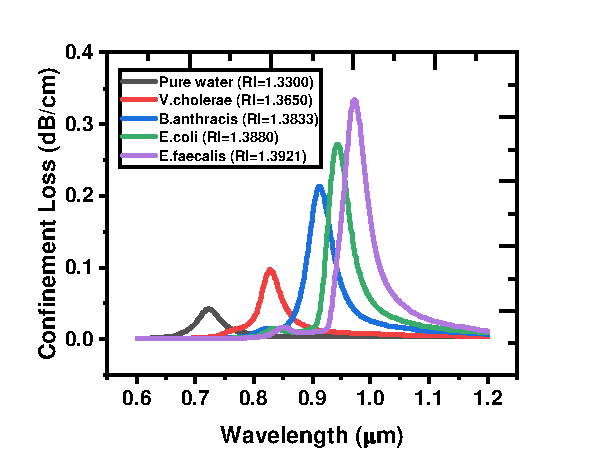
\includegraphics[width=0.5\textwidth]{Pathogen(main)_s.pdf}
    \caption{Confinement loss spectra of the proposed DLC-coated PCF-SPR sensor for different waterborne pathogens.}
    \label{fig:pathogen_cl_dlc}
\end{figure}

Figure~\ref{fig:pathogen_cl_dlc} shows the confinement loss spectra of the proposed DLC-coated sensor for the selected water pathogen samples. From the figure, it is clearly observed that the resonance peak moves toward the longer wavelength region when the refractive index of the sample increases. For pure water, the resonance peak appears near 0.72~\textmu m. For \textit{V. cholerae}, \textit{B. anthracis}, \textit{E. coli}, and \textit{E. faecalis}, the resonance peaks are found around 0.83~\textmu m, 0.91~\textmu m, 0.94~\textmu m, and 0.97~\textmu m, respectively. This gradual peak shifting indicates that the proposed sensor can detect different pathogen samples based on their RI-dependent resonance positions.

It is also seen that each pathogen sample produces a separate confinement loss peak. This is important for practical sensing because separated peaks make it easier to identify different water samples. The peak intensity also changes with the change of RI, which indicates that the interaction between the guided light and the sensing layer varies for different pathogen samples. Therefore, both the resonance wavelength position and the confinement loss response can be used to analyze the sensing behavior of the proposed sensor.

The sensing performance of the DLC-coated sensor for different water samples is summarized in Table~\ref{tab:pathogen_performance}. The resonance wavelength increases from 0.72~\textmu m to 0.97~\textmu m as the refractive index increases from 1.3300 to 1.3921. This 
\begin{table}[!t]
\centering
\caption{Performance analysis of the proposed DLC-coated sensor for water pathogen detection using pathogen RI values reported in \cite{deepti2025pcf}}
\label{tab:pathogen_performance}
\renewcommand{\arraystretch}{1.15}
\setlength{\tabcolsep}{2.5pt}
\scriptsize
\resizebox{\textwidth}{!}{%
\begin{tabular}{|l|c|c|c|c|c|c|c|}
\hline
\textbf{Water sample} & \textbf{RI} &
$\boldsymbol{\lambda_{\mathrm{res}}}$ &
\textbf{WS} & \textbf{AS} & \textbf{FWHM} & \textbf{FOM} & \textbf{Resolution} \\
 &  &
\textbf{(\textmu m)} &
\textbf{(nm/RIU)} &
\textbf{(RIU$^{-1}$)} &
\textbf{(\textmu m)} &
\textbf{(RIU$^{-1}$)} &
\textbf{(RIU)} \\
\hline
Pure water & 1.3300 & 0.72 & 3142.86 & -521.09 & 0.05 & 62.86 & $3.18\times10^{-5}$ \\
\hline
\textit{V. cholerae} & 1.3650 & 0.83 & 4371.58 & -864.18 & 0.04 & 109.29 & $2.29\times10^{-5}$ \\
\hline
\textit{B. anthracis} & 1.3833 & 0.91 & 6382.98 & -544.25 & 0.05 & 127.66 & $1.57\times10^{-5}$ \\
\hline
\textit{E. coli} & 1.3880 & 0.94 & 7317.07 & -581.69 & 0.04 & 182.93 & $1.37\times10^{-5}$ \\
\hline
\textit{E. faecalis} & 1.3921 & 0.97 & -- & -- & 0.04 & -- & -- \\
\hline
\end{tabular}%
}
\end{table}
confirms that the proposed sensor can effectively respond to small RI variations in water-based biological samples. The wavelength sensitivity, amplitude sensitivity, FWHM, FOM, and resolution are calculated from the corresponding confinement loss spectra. The obtained results indicate that the proposed DLC-coated PCF-SPR sensor can be applied for water pathogen detection through resonance wavelength monitoring.



To reduce the need for repeated full-wave simulation at every pathogen RI, a machine-learning-assisted prediction step is added after the numerical sensing analysis. The training dataset is formed from the DLC-coated confinement loss spectra simulated over the RI range of 1.33--1.40. Each spectrum is sampled at 61 wavelength points from 0.60 to 1.20~\textmu m. Thus, the input of the regression model is the analyte RI, $n_a$, and the output is the complete confinement loss curve, $\alpha(\lambda,n_a)$. The four pathogen RI values 1.3650, 1.3833, 1.3880, and 1.3921 are used as held-out testing samples, while RI = 1.3300 is already included in the reference simulation grid.

Gaussian process regression (GPR) is selected because the available training set is very small and the model can still learn a smooth nonlinear relation without requiring a large number of samples. The GPR models are implemented using the \texttt{GaussianProcessRegressor} module of scikit-learn with standardized RI input, output normalization, an RBF covariance kernel, and a white-noise term \cite{pedregosa2011scikit}. In GPR, the unknown response function is considered as a Gaussian process \cite{rasmussen2006gaussian},
\begin{equation}
f(n_a)\sim \mathcal{GP}\left(m(n_a),k(n_a,n_a')\right),
\label{eq:gpr_prior}
\end{equation}
where $m(n_a)$ is the mean function and $k(n_a,n_a')$ is the covariance kernel. In this work, a squared-exponential kernel is used to describe the smooth RI-dependent variation of the sensor response \cite{rasmussen2006gaussian},
\begin{equation}
k(n_a,n_a')=\sigma_f^2\exp\left[-\frac{(n_a-n_a')^2}{2l^2}\right]+\sigma_n^2\delta_{n_a n_a'},
\label{eq:gpr_kernel}
\end{equation}
where $\sigma_f^2$ is the signal variance, $l$ is the length scale, $\sigma_n^2$ is the noise term, and $\delta_{n_a n_a'}$ is the Kronecker delta. The direct GPR model learns the mapping $n_a\rightarrow [\alpha_1,\alpha_2,\ldots,\alpha_{61}]$ from the simulated curves.

However, direct curve prediction is not the most suitable form for this sensor response. In the direct GPR model, each wavelength point is treated as a fixed output column. For example, the model tries to learn the loss value at 0.90~\textmu m, 0.91~\textmu m, 0.92~\textmu m, and so on as separate outputs. This becomes difficult because the resonance peak does not stay at the same wavelength when the RI changes. A wavelength point that is located before the peak for one RI may become the peak region for another RI and may move to the falling side of the curve for a higher RI. Therefore, the value at a fixed wavelength can change suddenly, not because the sensor response is random, but because the whole peak is shifting along the wavelength axis. In other words, the direct model is forced to learn peak movement and curve shape at the same time from only a few training samples.

To make the learning problem simpler, a peak-aligned GPR model is also developed. The main idea is to first place all spectra in a common coordinate system where the resonance peak is located at zero and the peak height is normalized to one. After this transformation, the model no longer has to learn a moving peak as a moving object. Instead, it learns three simpler RI-dependent quantities: where the peak should be placed, how high the peak should be, and what the normalized spectral shape should look like. First, the resonance wavelength and peak loss are extracted from each training spectrum as
\begin{equation}
\lambda_p(n_a)=\arg\max_{\lambda}\alpha(\lambda,n_a), \qquad
A_p(n_a)=\max_{\lambda}\alpha(\lambda,n_a).
\label{eq:peak_extract}
\end{equation}
Then each curve is shifted and normalized using
\begin{equation}
\tilde{\lambda}=\lambda-\lambda_p(n_a), \qquad
\tilde{\alpha}(\tilde{\lambda},n_a)=\frac{\alpha(\lambda,n_a)}{A_p(n_a)}.
\label{eq:peak_align}
\end{equation}
This separates the prediction into three simpler parts: peak position, peak height, and normalized spectral shape. In the implementation, these three quantities are not predicted by three independent models. Instead, two multi-output GPR regressors are used: the first GPR regressor predicts the two peak parameters, $\lambda_p$ and $\log(A_p)$, while the second GPR regressor predicts the aligned normalized spectral shape. The final confinement loss curve is then restored as
\begin{equation}
\hat{\alpha}(\lambda,n_a)=\exp(\hat{z}_p)\,
\hat{s}\left(\lambda-\hat{\lambda}_p\right),
\label{eq:peak_restore}
\end{equation}
where $\hat{\lambda}_p$ is the predicted resonance wavelength, $\hat{z}_p=\log(\hat{A}_p)$ is the predicted logarithmic peak loss, and $\hat{s}$ is the predicted normalized shape. This alignment idea is consistent with curve registration and landmark-based alignment, where identifiable features such as peaks are used to reduce phase or position variation before comparing functional responses \cite{ramsay2005functional,ramsay1998curve,james2007curve,marron2015functional}.

\begin{figure}[!t]
    \centering
    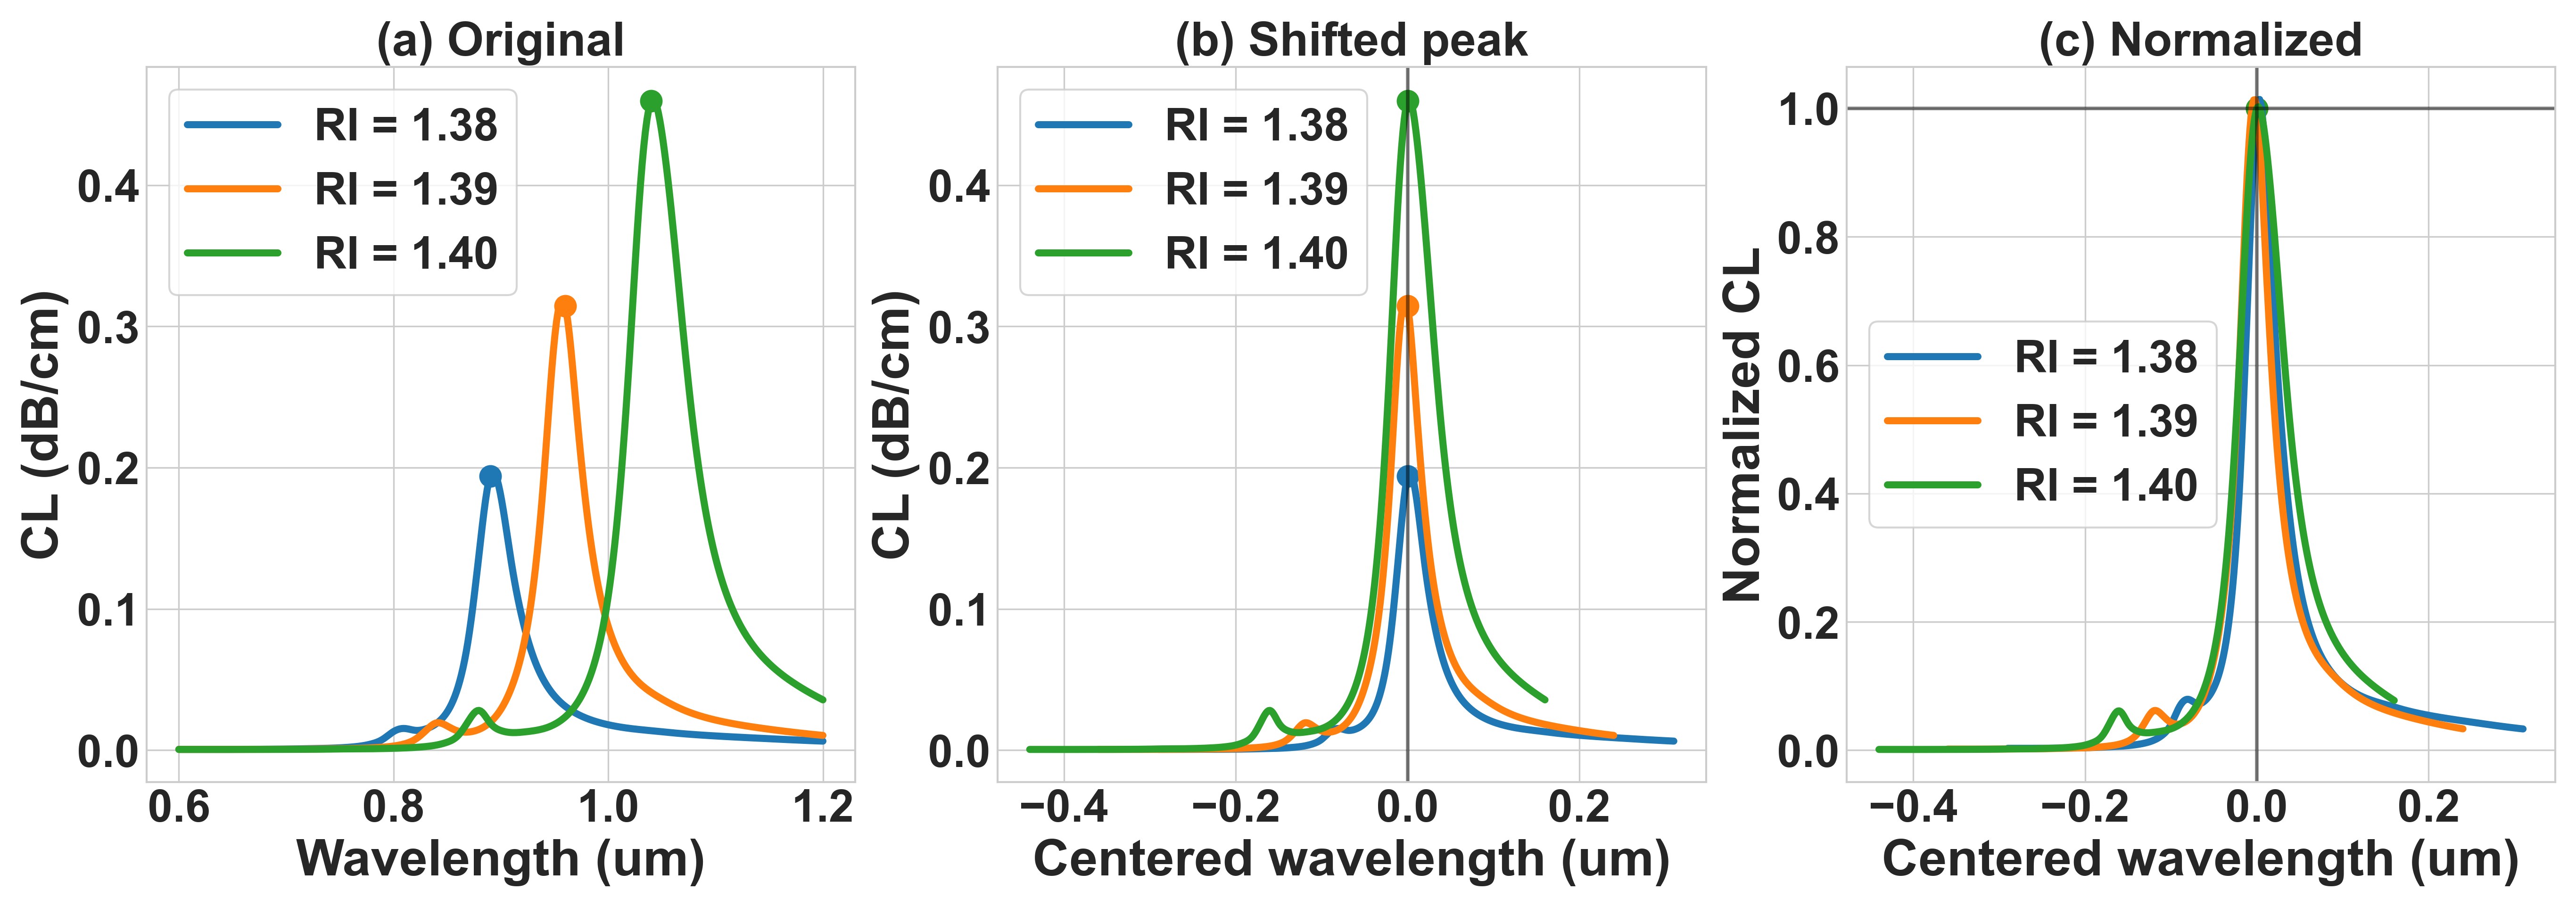
\includegraphics[width=1.0\textwidth]{ML_peak_alignment.png}
    \caption{Peak-alignment procedure used before GPR prediction: (a) original CL spectra, (b) shifted spectra with resonance peaks moved to zero wavelength offset, and (c) normalized spectra after dividing by the peak CL, where CL denotes confinement loss.}
    \label{fig:ml_peak_alignment}
\end{figure}

The testing performance of the direct GPR and peak-aligned GPR models is summarized in Table~\ref{tab:ml_model_comparison}. The direct GPR model gives an overall $R^2$ of 0.7137, with MAE and RMSE values of 0.01485 and 0.02995, respectively. This result shows that the direct model can follow the general trend, but it loses accuracy near the resonance peaks. After applying peak alignment, the overall $R^2$ increases to 0.9801, while the MAE and RMSE decrease to 0.00305 and 0.00791, respectively. The mean resonance wavelength error is also reduced from 0.0175~\textmu m to 0.0025~\textmu m. Therefore, the improvement is not only numerical; it directly improves the prediction of the physical resonance point of the sensor.

\begin{table}[!t]
\centering
\caption{Testing performance comparison between direct GPR and peak-aligned GPR.}
\label{tab:ml_model_comparison}
\renewcommand{\arraystretch}{1.35}
\setlength{\tabcolsep}{6pt}
\small
\resizebox{\textwidth}{!}{%
\begin{tabular}{|l|c|c|c|c|c|}
\hline
\textbf{Model} & $\boldsymbol{R^2}$ & \textbf{MAE} & \textbf{RMSE} &
\begin{tabular}[c]{@{}c@{}}\textbf{Mean peak WL}\\\textbf{error (\textmu m)}\end{tabular} &
\begin{tabular}[c]{@{}c@{}}\textbf{Mean peak CL}\\\textbf{error}\end{tabular} \\
\hline
Direct GPR & 0.7137 & 0.01485 & 0.02995 & 0.0175 & 0.03640 \\
\hline
Peak-aligned GPR & 0.9801 & 0.00305 & 0.00791 & 0.0025 & 0.01301 \\
\hline
\end{tabular}%
}
\end{table}

Table~\ref{tab:ml_peak_prediction} gives the peak-level comparison for the four held-out pathogen RI samples. For direct GPR, the predicted peak wavelength deviates by 0.01--0.02~\textmu m because the model predicts all fixed wavelength points at once. The peak-aligned GPR model gives exact peak wavelength prediction for three of the four testing samples and only 0.01~\textmu m error for RI = 1.3833. The peak loss values are also closer to the actual simulated values for all four samples. This confirms that peak alignment helps the model learn the resonance movement instead of treating it as an irregular point-by-point change in the output curve.

\begin{table}[!t]
\centering
\caption{Actual and predicted resonance peak values for the held-out pathogen RI samples.}
\label{tab:ml_peak_prediction}
\renewcommand{\arraystretch}{1.18}
\setlength{\tabcolsep}{3pt}
\scriptsize
\resizebox{\textwidth}{!}{%
\begin{tabular}{|c|c|c|c|c|c|c|}
\hline
\multirow{2}{*}{\textbf{RI}} &
\multicolumn{2}{c|}{\textbf{Actual FEM result}} &
\multicolumn{2}{c|}{\textbf{Direct GPR}} &
\multicolumn{2}{c|}{\textbf{Peak-aligned GPR}} \\
\cline{2-7}
& $\boldsymbol{\lambda_p}$ \textbf{(\textmu m)} & $\boldsymbol{A_p}$ &
$\boldsymbol{\hat{\lambda}_p}$ \textbf{(\textmu m)} & $\boldsymbol{\hat{A}_p}$ &
$\boldsymbol{\hat{\lambda}_p}$ \textbf{(\textmu m)} & $\boldsymbol{\hat{A}_p}$ \\
\hline
1.3650 & 0.83 & 0.10298 & 0.85 & 0.08779 & 0.83 & 0.09742 \\
\hline
1.3833 & 0.91 & 0.22155 & 0.89 & 0.16042 & 0.92 & 0.21180 \\
\hline
1.3880 & 0.94 & 0.28252 & 0.96 & 0.29426 & 0.94 & 0.26804 \\
\hline
1.3921 & 0.97 & 0.35087 & 0.96 & 0.29334 & 0.97 & 0.32862 \\
\hline
\end{tabular}%
}
\end{table}

\begin{figure}[!t]
    \centering
    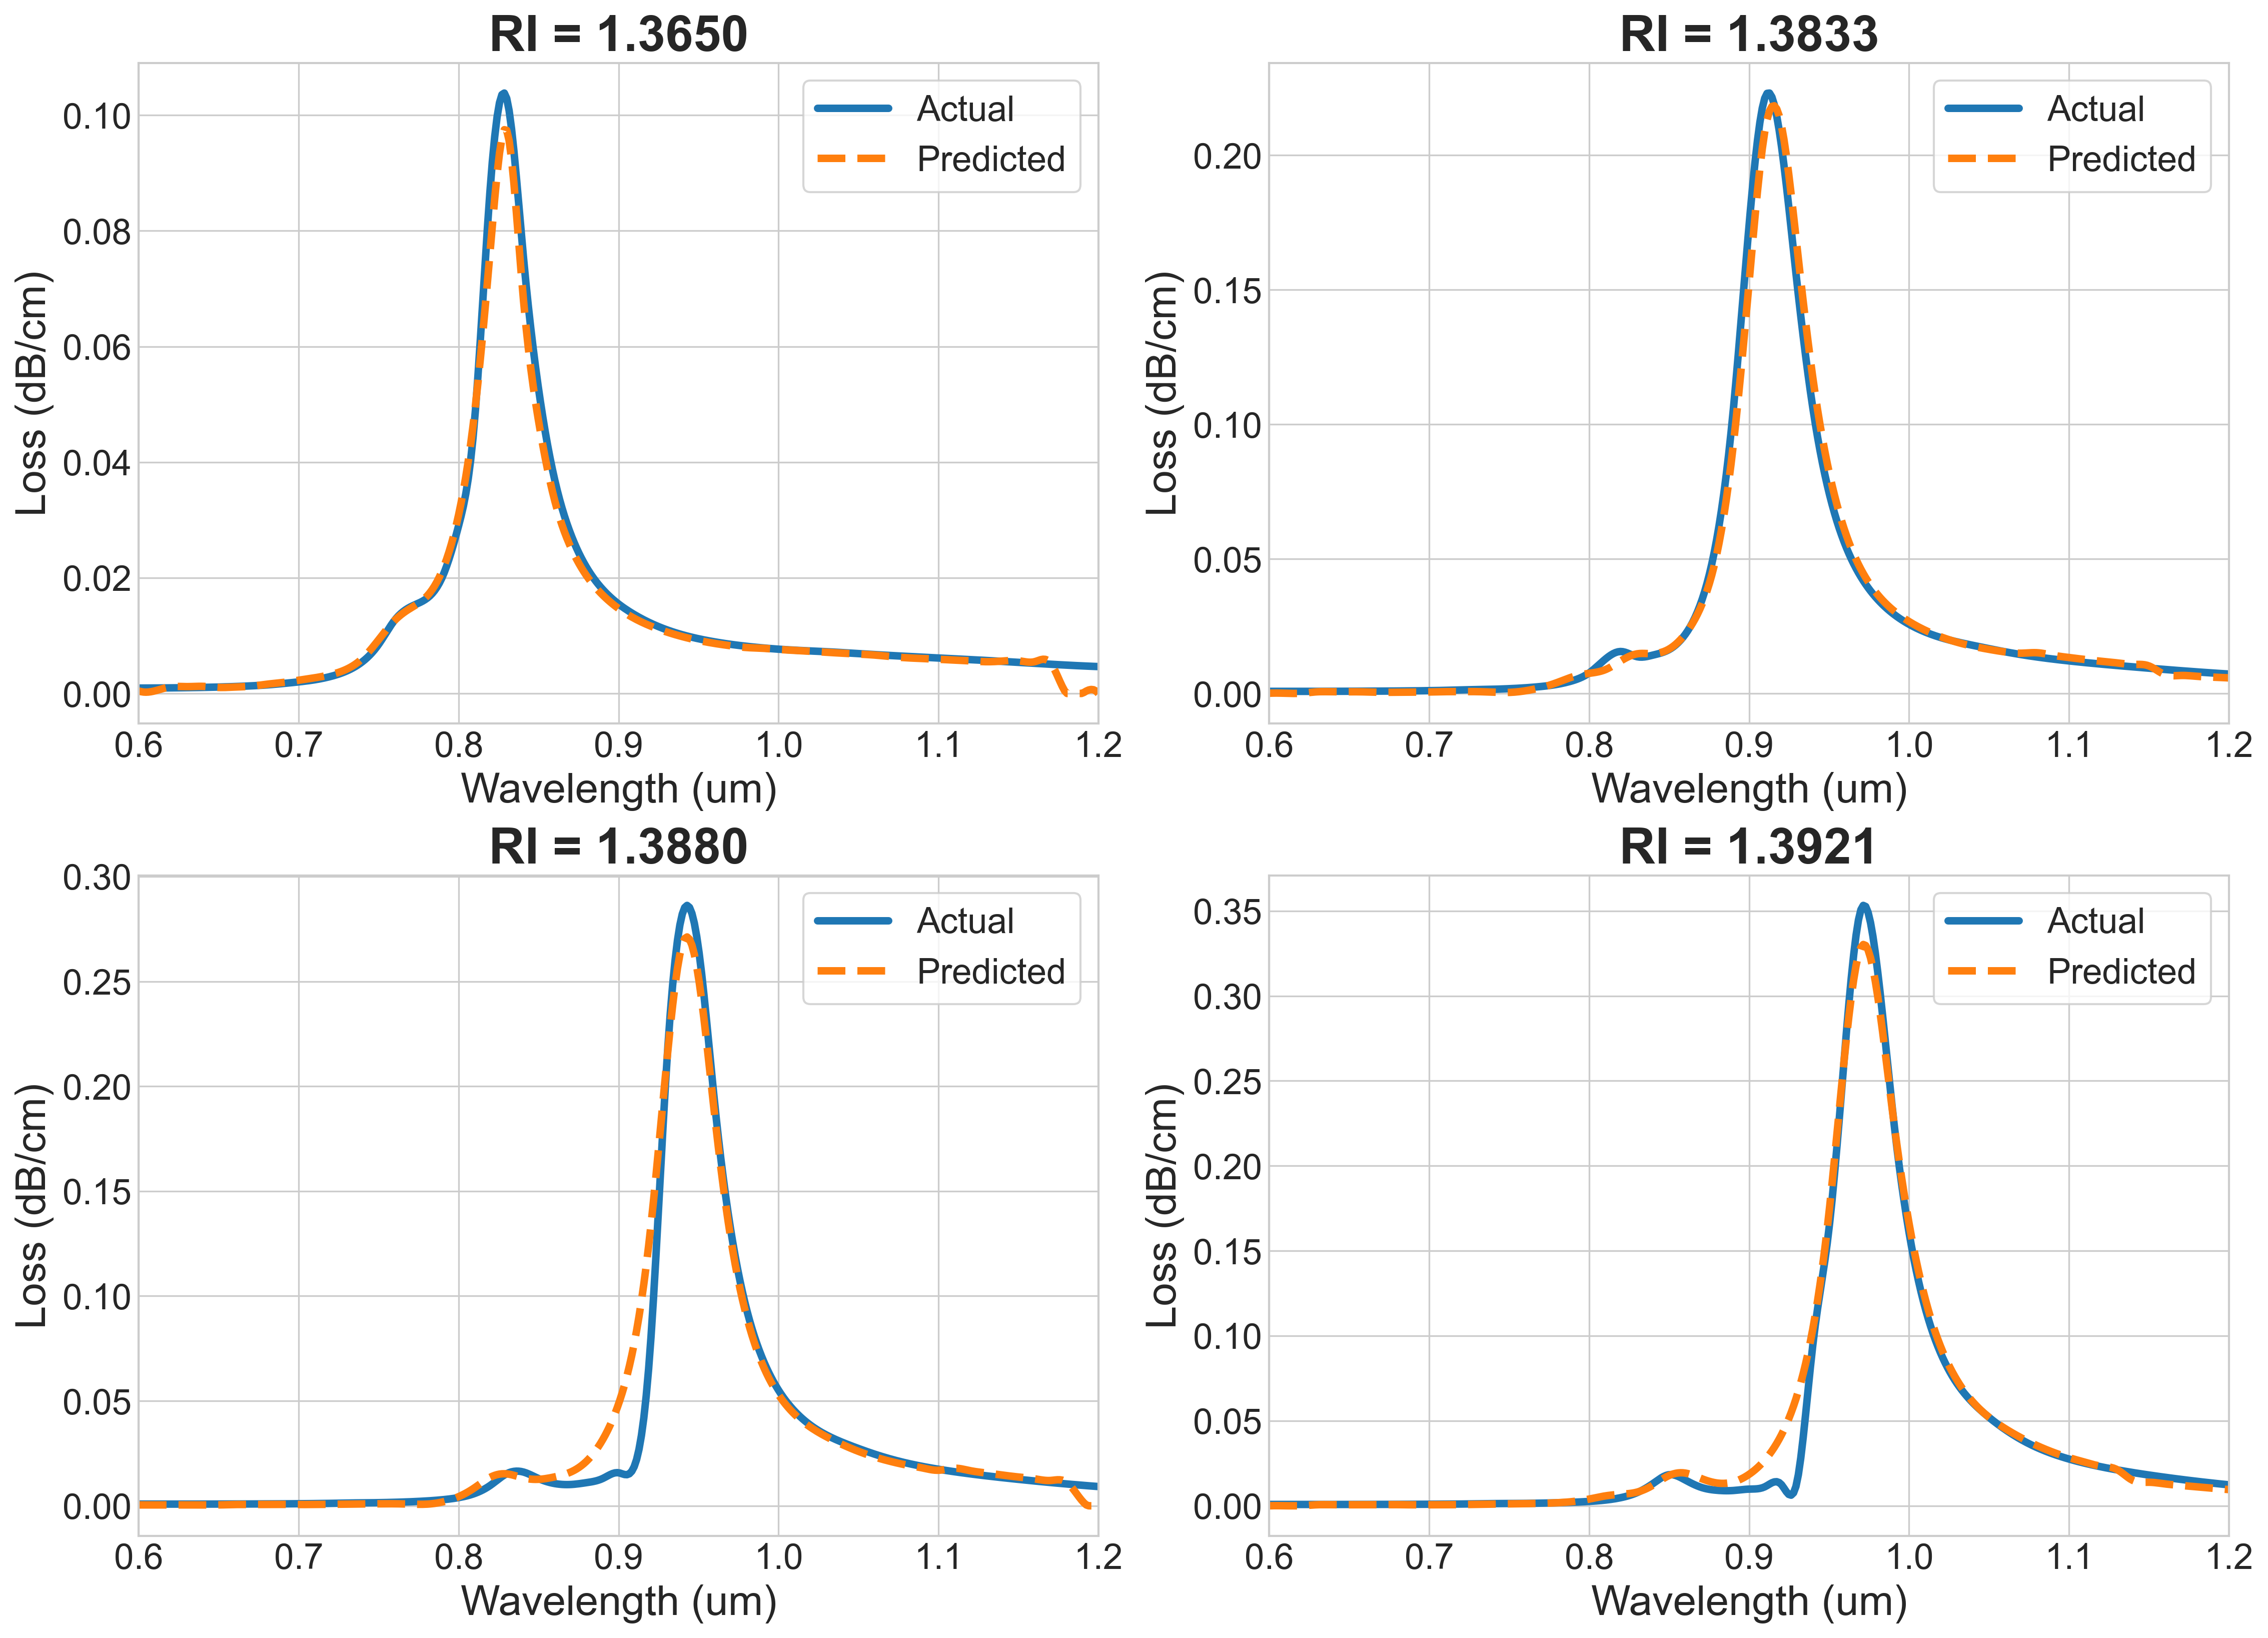
\includegraphics[width=1.0\textwidth]{ML_peak_aligned_gpr_prediction.png}
    \caption{Actual and predicted CL spectra for the held-out pathogen RI samples using the peak-aligned GPR model, where CL denotes confinement loss.}
    \label{fig:ml_peak_aligned_gpr_prediction}
\end{figure}

The overlay curves in Fig.~\ref{fig:ml_peak_aligned_gpr_prediction} show that the peak-aligned GPR model can reproduce both the spectral shift and the peak magnitude of the pathogen samples with good agreement. Some small difference remains in the tail region after the resonance peak, especially for the higher RI samples, because only eight simulated spectra are available for training. Even with this limited dataset, the model captures the main resonance behavior and gives reliable peak prediction. Hence, the peak-aligned GPR model is used here as a supporting prediction tool for rapid estimation of pathogen-specific sensor response, while the FEM simulation remains the reference source for final sensor validation.

\subsection{\textbf{{Fabrication Feasibility of the Proposed Biosensor}}}

The proposed PCF-SPR biosensor is compatible with fabrication approaches that have already been discussed for several closely related D-shaped and open-channel photonic crystal fibre platforms. Recent studies have reported open D-channel, slotted D-shaped, and partially etched D-shaped PCF configurations for cancer-related sensing applications, which indicates that the required microstructured fibre geometry is consistent with current design trends in plasmonic PCF biosensors \cite{ashrafian2025highly,bhuyan2025black,singh2023bottom}. In particular, the stack-and-draw method remains a practical route for arranging capillaries with different structural roles, after which controlled post-processing can be used to obtain the exposed sensing region required for plasmonic interaction \cite{ashrafian2025highly}.

After the fibre structure is formed, the sensing interface can be developed through selective polishing, partial etching, or microchannel formation, depending on the final architecture of the device. Related studies have shown that locating the sensing region on an exposed or partially opened surface brings the analyte closer to the fibre core and reduces the area that must be coated with functional materials \cite{ashrafian2025highly,singh2023bottom,rafi2025cancer}. This localised strategy is advantageous from a manufacturing perspective because it lowers material consumption and simplifies the coating process compared with full-surface deposition \cite{ashrafian2025highly,rafi2025cancer}.

The deposition stage is also supported by existing literature on comparable PCF-SPR structures. Multilayer configurations based on Au-TiO$_2$, Au-Ta$_2$O$_5$, black-phosphorus-assisted coatings, and Au-TiO$_2$-DLC have already been explored in closely related sensor designs, suggesting that selective functionalisation of the active sensing zone is technically feasible \cite{rafi2025cancer,bhuyan2025black,erdogan2025diamond}. Moreover, microchannel-based structures have been associated with atomic layer deposition for coating the sensing region, while DLC-assisted designs have been linked with PECVD-based thin-film preparation, supporting the use of controlled deposition techniques for producing stable and uniform nanolayers \cite{ashrafian2025highly,erdogan2025diamond}.

From an operational point of view, sample handling is also practically achievable. In partially etched D-shaped PCF biosensors, liquid samples have been considered for introduction into the sensing region through capillaries or suction-assisted flow mechanisms \cite{singh2023bottom}. Therefore, the proposed biosensor can reasonably be regarded as fabrication-feasible within the framework of current PCF processing, surface modification, and thin-film coating strategies reported for related SPR-based cancer sensing platforms \cite{ashrafian2025highly,bhuyan2025black,singh2023bottom,erdogan2025diamond,rafi2025cancer}.

\section{\textbf{{Conclusion}}}

In this work, a DLC-enhanced TiO$_2$-Au-coated slotted PCF-SPR sensor is proposed for wide-range refractive index detection. The sensor performance is numerically studied using the finite element method over the analyte RI range of 1.33--1.40. The optimized structural parameters are selected as TiO$_2$ thickness of 10 nm, Au thickness of 40 nm, DLC thickness of 10 nm, air-hole diameter of 3 $\mu$m, and pitch of 2.5 $\mu$m. The simulation results show that the addition of the DLC layer improves the sensing response in most of the investigated RI values. Compared with the structure without DLC, the DLC-coated sensor provides stronger wavelength shift, improved amplitude response, sharper resonance behaviour, higher FOM, and better resolution in most cases. The proposed sensor achieves a maximum wavelength sensitivity of 13000 nm/RIU, maximum amplitude sensitivity of $-1768.4$ RIU$^{-1}$, highest FOM of 216.67 RIU$^{-1}$, and minimum resolution of $7.7\times10^{-6}$ RIU. The comparative study also shows that the proposed sensor performs better than selected recently reported Au-based and TiO$_2$-Au-based SPR sensors in terms of maximum wavelength sensitivity and resolution. The improved performance is mainly due to the DLC layer, which enhances the interaction between the guided core mode and the plasmonic surface. Therefore, the proposed DLC-enhanced TiO$_2$-Au-coated PCF-SPR sensor can be a promising candidate for wide-range biomedical, chemical, and environmental RI sensing applications.


\bibliographystyle{elsarticle-num}
\bibliography{references}

%% else use the following coding to input the bibitems directly in the
%% TeX file.

%%\begin{thebibliography}{00}

%% \bibitem[Author(year)]{label}
%% For example:

%% \bibitem[Aladro et al.(2015)]{Aladro15} Aladro, R., Martín, S., Riquelme, D., et al. 2015, \aas, 579, A101


%%\end{thebibliography}

\end{document}
